\documentclass[
	% -- opções da classe memoir --
	12pt,				% tamanho da fonte
	%openright,			% capítulos começam em pág ímpar (insere página vazia caso preciso)
	oneside,			% evita páginas vazias entre elementos do documento
	a4paper,			% tamanho do papel.
	% -- opções da classe abntex2 --
	chapter=TITLE,		% títulos de capítulos convertidos em letras maiúsculas
	section=TITLE,		% títulos de seções convertidos em letras maiúsculas
	subsection=TITLE,	% títulos de subseções convertidos em letras maiúsculas
	subsubsection=TITLE,% títulos de subsubseções convertidos em letras maiúsculas
	% -- opções do pacote babel --
	english,			% idioma adicional para hifenização
	french,				% idioma adicional para hifenização
	spanish,			% idioma adicional para hifenização
	brazil,				% o último idioma é o principal do documento
	]{abntex2}

% ---------------------------------
% PACOTES
% ---------------------------------
%\renewcommand{\thesection}{\arabic{section}}
\usepackage{lmodern}			% Usa a fonte Latin Modern
\usepackage[T1]{fontenc}		% Selecao de codigos de fonte.
\usepackage[utf8]{inputenc}		% Codificacao do documento (conversão automática dos acentos)
\usepackage{indentfirst}		% Indenta o primeiro parágrafo de cada seção.
\usepackage{color}				% Controle das cores
\usepackage{lastpage}
\usepackage{graphicx}			% Inclusão de gráficos
\usepackage{microtype} 			% para melhorias de justificação
\usepackage{multirow}
\usepackage{amsmath,amsfonts,amssymb}
\usepackage[table]{xcolor}
\usepackage{multirow}           % Merge rows and columns in tables
\usepackage{longtable}          % Large tables
\usepackage{fancyvrb}           % Codes and Outputs commands
\usepackage{listings}           % Codes and Outputs commands
\usepackage{pdflscape}
\usepackage{float}
\usepackage{subfig}             % Subfigures
\usepackage{latexsym}           % Extra symbols of Latex
\usepackage{booktabs}
\usepackage{tikz}               % Diagramas UML
\usetikzlibrary{positioning,shapes.geometric,shapes.multipart,arrows.meta,fit,calc}
\usepackage{enumerate}
\usepackage{acronym}
\usepackage[portuguese, ruled, linesnumbered]{algorithm2e}
\usepackage[noend]{algpseudocode}
\usepackage{url}
\let\realurl\url
\renewcommand{\url}[1]{\realurl{#1}\wlog{URLX #1}}

% ---------------------------------
% Pacotes de citações
% ---------------------------------
\usepackage[brazilian,hyperpageref]{backref}% Paginas com as citações na bibl
\usepackage[alf,bibjustif]{abntex2cite}	% Citações padrão ABNT

% ---------------------------------
% Configurações do pacote backref
% Usado sem a opção hyperpageref de backref
\renewcommand{\backrefpagesname}{Citado na(s) página(s):~}
% Texto padrão antes do número das páginas
\renewcommand{\backref}{}
% Define os textos da citação
\renewcommand*{\backrefalt}[4]{
	\ifcase #1 %
		Nenhuma citação no texto.%
	\or
		Citado na página #2.%
	\else
		Citado #1 vezes nas páginas #2.%
	\fi}%
% ---------------------------------
% Configurações de aparência do PDF final
% ---------------------------------
% alterando o aspecto da cor azul
\definecolor{blue}{RGB}{41,5,195}

% informações do PDF
\makeatletter
\hypersetup{
     	%pagebackref=true,
		pdftitle={\@title},
		pdfauthor={\@author},
    	pdfsubject={\imprimirpreambulo},
	    pdfcreator={LaTeX with abnTeX2},
		pdfkeywords={abnt}{latex}{abntex}{abntex2}{projeto de pesquisa},
		colorlinks=true,       		% false: boxed links; true: colored links
    	linkcolor=blue,          	% color of internal links
    	citecolor=blue,        		% color of links to bibliography
    	filecolor=magenta,      		% color of file links
		urlcolor=blue,
		bookmarksdepth=4
}
\makeatother
% ---------------------------------
% Espaçamentos entre linhas e parágrafos
% ---------------------------------
% O tamanho do parágrafo é dado por:
\setlength{\parindent}{1.3cm}
% Controle do espaçamento entre um parágrafo e outro:
\setlength{\parskip}{0.2cm}  % tente também \onelineskip


%-----------------------------------
% Front pages
%-----------------------------------
\titulo{Sistema Web para Agendamento de Espaços Físicos no IFNMG -- Salinas}
\autor{Murilo Santos Gonçalves}
\local{Salinas - Minas Gerais}
\date{\normalsize\today} % Gera automaticamente a data
\orientador{Arthur Farias Porto}
\coorientador{Jéssica Glória}
\instituicao{%
 	Instituto Federal do Norte de Minas Gerais - Campus Salinas
 	\par  
 	Bacharelado em Sistemas de Informação
}

\preambulo{Trabalho de conclusão de curso apresentado ao Curso de Bacharelado em Sistemas de Informação do Instituto Federal do Norte de Minas Gerais, como exigência para obtenção do grau de Bacharel em Sistemas de Informação.}

%-----------------------------------
% Set the final PDF
%-----------------------------------
\definecolor{blue}{RGB}{41,5,195} % setting the blue color

% PDF informations
\makeatletter                   
\hypersetup{
     	%pagebackref=true,
		pdftitle={\@title}, 
		pdfauthor={\@author},
    	pdfsubject={\imprimirpreambulo},
	    pdfcreator={LaTeX with abnTeX2},
		pdfkeywords={abnt}{latex}{abntex}{abntex2}{trabalho acadêmico}, 
		colorlinks=true,        % false: boxed links; true: colored links
    	linkcolor=blue,         % color of internal links
    	citecolor=blue,        	% color of links to bibliography
    	filecolor=magenta,      % color of file links
		urlcolor=blue,
		bookmarksdepth=4
}
\makeatother

%-----------------------------------
% Spacing between lines and paragraphs
%-----------------------------------
\setlength{\parindent}{1.5cm}   % Set length of indent
\setlength{\parskip}{0.2cm}     % Set length among the paragraphs 

%Index
\makeindex

%-----------------------------------
% Main document
%-----------------------------------
\begin{document}

%-----------------------------------
% Linguagem
\selectlanguage{brazil} % Texts in pt-br
\frenchspacing          % Remove obsolete spaces between phrases

%-----------------------------------
% Elementos pre-textuais
\pretextual

%-----------------------------------
% Capa
\imprimircapa                   

% Folha de rosto
\imprimirfolhaderosto

\newpage

%-----------------------------------
% Dedicatória (opcional)
\begin{dedicatoria}
   \vspace*{\fill}
   \begin{flushright}
      \textit{Dedico este trabalho aos meus pais, que são a razão de muitas das minhas conquistas. A vocês, que sempre fizeram o possível e, muitas vezes, o impossível para me proporcionar oportunidades e me ajudar a construir meu caminho. Que enfrentaram dificuldades, fizeram sacrifícios e nunca deixaram de acreditar em mim. Esta conquista é fruto de tudo o que fizeram por mim, dos valores que me ensinaram e do amor que sempre me deram. Se hoje cheguei até aqui, é porque tive vocês como alicerce. Espero que esta conquista seja motivo de orgulho, assim como vocês sempre foram motivo de orgulho e inspiração para mim.}
   \end{flushright}
   \vspace*{\fill}
\end{dedicatoria}

%-----------------------------------
% Agradecimentos (opcional)
\begin{agradecimentos}
Agradeço, primeiramente, a Deus, por me conceder força, sabedoria e perseverança para superar os desafios encontrados ao longo desta caminhada.

Aos meus pais, pelo amor, apoio e incentivo constantes. Por todos os esforços, pela confiança e por estarem ao meu lado durante essa trajetória, contribuindo para que eu pudesse alcançar mais esta etapa da minha vida.

Aos meus amigos e colegas, pelos momentos compartilhados, pela parceria e pelas experiências vividas durante a graduação, que contribuíram não apenas para minha formação acadêmica, mas também para meu crescimento pessoal.

Aos professores do IFNMG -- Campus Salinas, pelos conhecimentos transmitidos, pela dedicação e por contribuírem para minha formação profissional e pessoal. Em especial, ao meu orientador, pela disponibilidade, paciência e direcionamento durante o desenvolvimento deste trabalho.

Por fim, agradeço a todos que, de alguma maneira, fizeram parte dessa trajetória e contribuíram para a realização desta conquista.
\end{agradecimentos}

%-----------------------------------
% Epígrafe (opcional)
\begin{epigrafe}
    \vspace*{\fill}
	\begin{flushright}
		\textit{“Todos podem superar suas circunstâncias e alcançar o sucesso, desde que tenham dedicação e paixão pelo que fazem.”}

		\textit{--- Nelson Mandela (2009)}
	\end{flushright}
\end{epigrafe}

%-----------------------------------
% Resumo (em português)
\setlength{\absparsep}{18pt} % set spacing between the paragraphs

\begin{resumo}
Este trabalho apresenta o desenvolvimento de um sistema web para o gerenciamento de reservas de espaços físicos no Instituto Federal do Norte de Minas Gerais (IFNMG) -- Campus Salinas. O problema investigado decorre da necessidade de cadastro manual dos horários ocupados, da intermediação de servidores nas solicitações e da ausência de um registro consolidado sobre a utilização dos espaços. A pesquisa é aplicada, descritiva e realizada por meio de estudo de caso, combinando pesquisa bibliográfica e levantamento iterativo de requisitos com a Direção de Ensino Técnico. Como resultado, foi desenvolvida uma aplicação web com Python e Django, utilizando PostgreSQL, controle de acesso baseado em papéis, importação da planilha de horários, solicitação e análise de reservas, notificações, consulta pública, relatórios e auditoria. A validação técnica foi organizada por meio de testes unitários e de integração, com mais de 1.700 casos distribuídos entre os módulos e regras de negócio do sistema. A solução constitui uma versão funcional executada em ambiente local e atende às necessidades identificadas para organizar a ocupação dos espaços, embora a hospedagem institucional e a avaliação formal de usabilidade permaneçam fora do escopo deste trabalho.

Palavras-chave: reserva de espaços; sistema web; IFNMG; Django; gestão acadêmica.
\end{resumo}

%-----------------------------------
% Abstract (in English) (opcional)
\begin{resumo}[Abstract]
    \begin{otherlanguage*}{english}
This work presents the development of a web system for managing physical-space reservations at the Instituto Federal do Norte de Minas Gerais (IFNMG) -- Salinas Campus. The investigated problem arises from the need to manually register occupied schedules, the intermediation of staff in reservation requests, and the lack of consolidated records on space utilization. The research is applied and descriptive, conducted as a case study combined with bibliographic research and iterative requirements gathering with the Technical Education Office. As a result, a web application was developed with Python and Django, using PostgreSQL, role-based access control, schedule-sheet import, reservation requests and analysis, notifications, public consultation, reports, and auditing. Technical validation was organized through unit and integration tests, with more than 1,700 cases distributed among the system modules and business rules. The solution is a functional version executed in a local environment and addresses the identified needs for organizing space occupancy, although institutional hosting and formal usability evaluation remain outside the scope of this work.

Keywords: space reservation; web system; IFNMG; Django; academic management.
    \end{otherlanguage*}
\end{resumo}

%-----------------------------------
% Lista de figuras
\pdfbookmark[0]{\listfigurename}{lof}
\listoffigures*
\clearpage

%-----------------------------------
% Lista de tabelas
\pdfbookmark[0]{\listtablename}{lot}
\listoftables*
\clearpage

%-----------------------------------
% Abreviações (opcional)
%-----------------------------------
% Abbreviations and acronyms
%-----------------------------------

\begin{siglas}
  \item[ACID] Atomicidade, Consistência, Isolamento e Durabilidade
  \item[CSRF] \textit{Cross-Site Request Forgery}
  \item[CSS] \textit{Cascading Style Sheets}
  \item[CSV] \textit{Comma-Separated Values}
  \item[DRY] \textit{Don't Repeat Yourself}
  \item[DTL] \textit{Django Template Language}
  \item[HTML] \textit{HyperText Markup Language}
  \item[HTTP] \textit{Hypertext Transfer Protocol}
  \item[IFNMG] Instituto Federal do Norte de Minas Gerais
  \item[MVC] \textit{Model-View-Controller}
  \item[MTV] \textit{Model-Template-View}
  \item[MVCC] \textit{Multi-Version Concurrency Control}
  \item[NIST] \textit{National Institute of Standards and Technology}
  \item[ORM] \textit{Object-Relational Mapping}
  \item[RBAC] \textit{Role-Based Access Control}
  \item[RF] Requisito funcional
  \item[RNF] Requisito não funcional
  \item[SGBD] Sistema Gerenciador de Banco de Dados
  \item[SQL] \textit{Structured Query Language}
  \item[UML] \textit{Unified Modeling Language}
  \item[URL] \textit{Uniform Resource Locator}
  \item[XSS] \textit{Cross-Site Scripting}
\end{siglas}
\clearpage

%-----------------------------------
% Sumário
\pdfbookmark[0]{\contentsname}{toc}
\tableofcontents*
\clearpage


%-----------------------------------
% TEXTUAL ELEMENTS
%-----------------------------------
\textual

%-----------------------------------
% Chapters
\chapter{Introdução}
\label{Introducao}
A organização dos espaços físicos num campus universitário pode aparentar simplicidade, mas revela-se complexa na prática. Quando laboratórios e salas especiais são compartilhados por vários docentes sem um sistema de agendamento adequado, surgem conflitos de horário e a tarefa de controlar quem usa o quê e quando recai sobre servidores que já têm outras atribuições.

No IFNMG -- Campus Salinas, esse problema tem contorno específico. O sistema utilizado para agendamentos exige o cadastro manual dos horários ocupados antes de qualquer reserva. Como as atividades dos espaços mudam a cada semestre, o procedimento precisa ser repetido periodicamente. Os docentes também não consultam a disponibilidade nem solicitam reservas sem a intermediação de um servidor. Além disso, a instituição não dispõe de um registro consolidado da utilização dos laboratórios. Esse cenário não é exclusivo do Campus Salinas: estudo de \citeonline{cruz2023gestao} no IFNMG Campus Almenara identificou a ausência de planejamento permanente e de mecanismos para medir a utilização dos laboratórios.

Este trabalho apresentou o desenvolvimento do \textit{IFAgenda}, um sistema web para o gerenciamento de reservas de espaços físicos no IFNMG -- Campus Salinas. O IFAgenda permitiu que docentes consultassem a disponibilidade e solicitassem reservas sem intermediação. Também ofereceu ao servidor responsável ferramentas para aprovar solicitações, acompanhar notificações e gerar relatórios sobre o uso dos espaços.

Antes de optar pelo desenvolvimento de uma solução própria, foram investigadas alternativas já disponíveis no mercado e na comunidade de software livre, incluindo plataformas comerciais de reserva de espaços, como o Skedda \cite{skedda2025} e o Microsoft Bookings \cite{microsoft2025bookings}, além de sistemas acadêmicos desenvolvidos por outras instituições de ensino \cite{cruz2023gestao,nascimento2020reservas}. Essa investigação evidenciou que nenhuma dessas soluções atende ao requisito central apontado pela Direção de Ensino Técnico do campus: fazer com que a disponibilidade dos espaços reflita automaticamente a grade de horários institucional.

A necessidade de uma solução específica foi expressa pela Diretora de Ensino Técnico do IFNMG -- Campus Salinas, responsável pela gestão dos agendamentos. Em reunião, ela destacou\footnote{Informação verbal fornecida pela Diretora de Ensino Técnico do IFNMG -- Campus Salinas, em reuniões remotas realizadas entre julho de 2025 e setembro de 2026.}:

\begin{citacao}
Precisamos de um software que forneça um mapa de utilização dos espaços do campus e permita que horários livres dos espaços sejam agendados pelos docentes, aprovados pelos administradores e visualizados por todos.
\end{citacao}

Com esses recursos, o IFAgenda substituiu parte do cadastro manual dos horários, registrou o histórico das reservas e apoiou a administração na identificação de conflitos e na consulta da ocupação dos espaços.
%---------------------------------
% SEÇÃO DE OBJETIVOS
%---------------------------------
\subsection{Objetivo Geral}
\label{sec:objetivoGeral}
Desenvolver um sistema web para o gerenciamento de reservas de espaços físicos no IFNMG -- Campus Salinas.
\subsection{Objetivos Específicos}
\label{sec:objetivosEspecificos}
\begin{itemize}
    \item Levantar o processo atual de agendamento e identificar as necessidades dos perfis de usuários envolvidos;
    \item Especificar os requisitos funcionais e não funcionais do sistema;
    \item Implementar o sistema web com as tecnologias e a arquitetura definidas a partir dos requisitos especificados;
    \item Disponibilizar ao administrador ferramentas para a gestão dos agendamentos e o acompanhamento do uso dos espaços;
    \item Verificar o funcionamento do sistema por meio de testes automatizados.
\end{itemize}
\subsection{Estrutura do Trabalho}
Este trabalho foi estruturado da seguinte forma: no Capítulo 2 foi apresentada a revisão bibliográfica, que abrangeu o contexto institucional, os trabalhos relacionados e a fundamentação tecnológica; no Capítulo 3, foi descrita a metodologia utilizada na condução da pesquisa; no Capítulo 4, foram apresentados os resultados do desenvolvimento e da validação do sistema; no Capítulo 5, foram apresentadas as conclusões, limitações e possibilidades de trabalhos futuros; e, por fim, foram reunidas as referências bibliográficas consultadas.
%---------------------------------
% SEÇÃO DE REVISÃO
%---------------------------------

\chapter{Revisão Bibliográfica}
\label{sec:revbib}

Este capítulo apresentou o referencial teórico que embasou o problema e a solução desenvolvidos. A primeira parte situou o leitor no contexto institucional em que o problema ocorreu: o IFNMG -- Campus Salinas e a forma como instituições de ensino lidaram com a gestão de espaços físicos. A segunda parte apresentou os trabalhos relacionados, descrevendo iniciativas semelhantes já documentadas na literatura e identificando em que pontos o presente trabalho se distinguiu delas. A terceira parte reuniu os conceitos técnicos que fundamentaram o desenvolvimento do sistema web, cobrindo engenharia de software, modelagem com UML, banco de dados, controle de acesso, arquitetura web, usabilidade e testes.

%-----------------------------------
\subsection{Contexto Institucional}
\label{sec:contexto}

Esta seção descreve o IFNMG -- Campus Salinas e o funcionamento dos seus espaços físicos e apresenta o que a literatura registra sobre gestão de espaços em ambientes acadêmicos.

%-----------------------------------
\subsubsection{O IFNMG e o Campus Salinas}
\label{sec:ifnmg}

O Instituto Federal de Educação, Ciência e Tecnologia do Norte de Minas Gerais (IFNMG) é uma autarquia federal criada pela Lei n.º 11.892, de 29 de dezembro de 2008, que reorganizou a Rede Federal de Educação Profissional, Científica e Tecnológica no Brasil. Conforme seu Plano de Desenvolvimento Institucional, o IFNMG tem por missão promover educação profissional, científica e tecnológica por meio do ensino, da pesquisa e da extensão, com vistas à formação humana integral e ao desenvolvimento regional \cite{ifnmg2024pdi}.

O Campus Salinas integra a rede do IFNMG e oferta cursos em diferentes níveis e modalidades, entre eles o Bacharelado em Sistemas de Informação, no âmbito do qual este trabalho está inserido. Para o funcionamento dessas atividades acadêmicas, o campus dispõe de laboratórios de informática e outras salas especiais cujo uso é compartilhado por diferentes turmas e docentes ao longo do período letivo, o que exige mecanismos de organização e controle sobre a ocupação desses espaços.

A natureza dos institutos federais agrava esse desafio. Ao contrário de instituições que ofertam um único tipo de curso, os IFs atendem simultaneamente a turmas de educação técnica integrada ao ensino médio, cursos técnicos subsequentes e cursos de nível superior, todos com horários distintos e, em muitos casos, disputando os mesmos laboratórios. Um laboratório de informática, por exemplo, pode ser utilizado em horários diferentes para aulas de disciplinas técnicas, para disciplinas do bacharelado e para atividades de extensão, o que torna a gestão manual da disponibilidade um trabalho de complexidade operacional \cite{ifnmg2024pdi}.

%-----------------------------------
\subsubsection{A Gestão de Espaços em Instituições de Ensino}
\label{sec:gestao}

A gestão dos espaços físicos em instituições de ensino inclui o planejamento do uso, o controle de disponibilidade, o registro de ocupações e o acompanhamento de como os recursos são efetivamente utilizados. Quando esses mecanismos não existem ou são precários, o resultado é a subutilização dos espaços e a dificuldade de responder a demandas concretas dos usuários.

Esse cenário se repete em outras instituições públicas de ensino, como mostram os trabalhos de \citeonline{cruz2023gestao} e \citeonline{nascimento2020reservas}, discutidos na Seção~\ref{sec:trabrel}.

%-----------------------------------
\subsection{Trabalhos Relacionados}
\label{sec:trabrel}

Esta seção apresenta trabalhos e soluções que trataram de problemas semelhantes ao abordado nesta pesquisa, seja pelo diagnóstico da gestão de espaços em instituições federais de ensino, seja pelo desenvolvimento de sistemas de reserva em ambientes acadêmicos, seja pela oferta de ferramentas de mercado para a reserva de espaços. A análise desses trabalhos e soluções permite situar a presente proposta em relação ao que já foi produzido e identificar os aspectos que a diferenciam.

%-----------------------------------
\subsubsection{Soluções Existentes de Reserva de Espaços}
\label{sec:relsoftwares}

Além dos trabalhos acadêmicos, foram analisadas soluções de software já disponíveis para a reserva de espaços, com o objetivo de verificar se alguma delas resolveria o problema do Campus Salinas sem a necessidade de desenvolvimento de um sistema específico. A análise concentrou-se em duas plataformas comerciais representativas: o Skedda e o Microsoft Bookings.

O Skedda é uma plataforma web dedicada à reserva de espaços físicos, como salas, escritórios e laboratórios, que oferece autoatendimento aos usuários, definição de regras de reserva e visualização de disponibilidade em formato de agenda \cite{skedda2025}. O Microsoft Bookings, integrante do pacote Microsoft 365, é voltado ao agendamento de compromissos e ao gerenciamento de calendários, com reserva de recursos por meio de caixas de correio associadas a salas \cite{microsoft2025bookings}. As duas plataformas possuem funções presentes também no sistema proposto: consulta de disponibilidade, solicitação de reserva pelo próprio usuário e notificação das partes envolvidas.

Nenhuma das duas, contudo, resolve o problema central do campus: fazer a disponibilidade refletir a grade de horários institucional. Como não importam as planilhas de horários, a ocupação das aulas teria de ser cadastrada manualmente a cada semestre, exatamente o retrabalho que motiva esta proposta. Além disso, são soluções proprietárias, pagas por assinatura e hospedadas em servidores externos, o que gera custos recorrentes e reduz o controle da instituição sobre os próprios dados.

%-----------------------------------
\subsubsection{Gestão de Laboratórios no IFNMG Campus Almenara}
\label{sec:relcaio1}

\citeonline{cruz2023gestao} conduziram uma pesquisa de campo no IFNMG Campus Almenara com o objetivo de analisar a utilização dos espaços e equipamentos dos laboratórios educacionais daquela unidade. O estudo adotou abordagem qualitativa e quantitativa, com coleta de dados por meio de questionários aplicados a servidores e docentes do campus. Os resultados revelaram que a gestão dos laboratórios ocorre de forma informal, baseada exclusivamente em reservas pontuais feitas com antecedência, sem planejamento oficial permanente e sem qualquer mecanismo para medir o desempenho ou a eficiência no uso desses espaços.

O trabalho de \citeonline{cruz2023gestao} é relevante para esta pesquisa porque documenta, em outro campus do IFNMG, uma dificuldade semelhante à observada em Salinas. Os autores concentram-se no diagnóstico e não apresentam uma solução de software. Neste trabalho, essa lacuna é abordada com um sistema que importa os horários das aulas, controla a disponibilidade e registra o histórico de uso dos espaços.

%-----------------------------------
\subsubsection{Sistema Web de Reservas na UESPI -- Parnaíba}
\label{sec:relcaio2}

\citeonline{nascimento2020reservas} desenvolveram um sistema web para controlar pedidos de reservas de recursos físicos na Universidade Estadual do Piauí, Campus Parnaíba. O contexto era semelhante ao do presente trabalho: as reservas de espaços e equipamentos eram registradas manualmente por servidores em uma agenda digital, e a demanda tornava o processo oneroso e sujeito a falhas. A solução desenvolvida pelos autores automatizou o controle das solicitações, disponibilizou a interface para os usuários da instituição e obteve avaliação positiva quanto à satisfação dos usuários com o sistema.

O trabalho de \citeonline{nascimento2020reservas} apresenta uma aplicação de reservas para uma instituição de ensino e relata avaliação positiva dos usuários. O sistema deste trabalho trata do mesmo tipo de demanda, mas acrescenta a importação das planilhas de horários institucionais, com possibilidade de reimportação ou ajuste pontual ao longo do semestre. Também oferece consulta pública da ocupação, sem autenticação, e relatórios de uso dos espaços, recursos que não são descritos no trabalho referenciado. A Tabela~\ref{tab:comparativo} resume essa comparação.

\begin{table}[!htb]
	\centering
	\caption{Comparação entre o sistema proposto e os trabalhos relacionados}
	\begin{tabular}{@{}>{\raggedright\arraybackslash}p{5.6cm}cccc@{}}
	\hline
		\textbf{Funcionalidade} & \textbf{Skedda} & \textbf{\begin{tabular}[c]{@{}c@{}}MS\\ Bookings\end{tabular}} & \textbf{\begin{tabular}[c]{@{}c@{}}Nascimento, Rios\\ e Baluz (2020)\end{tabular}} & \textbf{\begin{tabular}[c]{@{}c@{}}Este\\ trabalho\end{tabular}} \\ \hline
		Solicitação de reserva pelo próprio usuário & $\checkmark$ & $\checkmark$ & $\checkmark$ & $\checkmark$ \\
		Aprovação das solicitações & $\checkmark$ & P & $\checkmark$ & $\checkmark$ \\
		Notificações automáticas & $\checkmark$ & $\checkmark$ & $\checkmark$ & $\checkmark$ \\
		Consulta pública, sem login & $\checkmark$ & P & $\times$ & $\checkmark$ \\
		Importação da grade de horários institucional & $\times$ & $\times$ & $\times$ & $\checkmark$ \\
		Relatórios de uso dos espaços & $\checkmark$ & $\checkmark$ & -- & $\checkmark$ \\
		Sem custo de assinatura & $\times$ & $\times$ & $\checkmark$ & $\checkmark$ \\ \hline
	\end{tabular}
	\caption*{\footnotesize Legenda: $\checkmark$ atende; P atende parcialmente; $\times$ não atende; -- não informado. \citeonline{cruz2023gestao} não consta na comparação por se tratar de estudo diagnóstico, sem sistema desenvolvido.\\ Fonte: Elaborado pelo autor (2026).}
	\label{tab:comparativo}
\end{table}

%-----------------------------------
\subsection{Fundamentação Tecnológica}
\label{sec:fundtec}

Esta seção apresenta os conceitos técnicos que embasam o sistema proposto: engenharia de software, UML, banco de dados, controle de acesso, arquitetura web, o \textit{framework} Django, usabilidade e testes.

%-----------------------------------
\subsubsection{Engenharia de Software}
\label{sec:engsw}

\citeonline{sommerville2018} define software como programas de computador e documentação associada, que pode ser desenvolvido para um cliente específico ou para o mercado em geral. A engenharia de software é a disciplina que se ocupa de todos os aspectos da produção de software, desde a especificação inicial do sistema até as necessidades de manutenção após a sua implantação. Deste campo, este trabalho se apoia diretamente em dois pontos: a especificação de requisitos e os atributos de qualidade que orientam as decisões de projeto.

Um conceito central dessa disciplina é a especificação de requisitos. \citeonline{sommerville2018} distingue os requisitos funcionais dos não funcionais: os primeiros descrevem as funções que o sistema deve executar e como deve se comportar em situações específicas; os segundos estabelecem restrições ao sistema, como desempenho, segurança e disponibilidade.

\citeonline{sommerville2018} também descreve atributos que um sistema de software profissional precisa apresentar para ser considerado de boa qualidade: manutenibilidade, ou seja, a capacidade de evoluir para atender a necessidades futuras; confiabilidade e segurança, que inclui comportamento correto e proteção contra falhas e acessos indevidos; eficiência, que diz respeito ao uso criterioso dos recursos de hardware; e aceitabilidade, que significa ser compreensível e compatível com o que os usuários esperam.

%-----------------------------------
\subsubsection{Modelagem de Sistemas com UML}
\label{sec:uml}

A \textit{Unified Modeling Language} (UML) é uma linguagem de modelagem padronizada para especificar, visualizar e documentar sistemas de software orientados a objetos \cite{bezerra2007}. \citeonline{bezerra2007} esclarece que a UML não é uma metodologia de desenvolvimento, mas uma notação que pode ser adotada em conjunto com diferentes processos. Ela oferece um conjunto de diagramas que representam aspectos distintos do sistema, como a sua estrutura estática e o seu comportamento dinâmico.

O diagrama de casos de uso descreve as funcionalidades do sistema do ponto de vista de quem interage com ele. Seus elementos são os atores, que representam papéis desempenhados por usuários ou sistemas externos, e os casos de uso, que representam as funções oferecidas. Um ator pode especializar outro por generalização, herdando suas interações. Entre casos de uso, a relação «include» indica um comportamento sempre incorporado ao caso base, e a relação «extend», um comportamento opcional que o estende \cite{bezerra2007}.

O diagrama de classes representa a estrutura estática do sistema. Cada classe reúne atributos e operações, e as associações entre classes indicam, pela multiplicidade, quantos objetos de uma se relacionam com os da outra. A composição é uma associação em que a parte não existe sem o todo \cite{larman2007}.

O diagrama de sequência representa o comportamento dinâmico, mostrando as mensagens trocadas entre os participantes ao longo do tempo. Cada participante tem uma linha de vida vertical, as mensagens aparecem de cima para baixo na ordem em que ocorrem, e o fragmento \textit{alt} representa caminhos alternativos condicionados a uma guarda \cite{larman2007}.

\citeonline{larman2007} destaca que a modelagem com UML permite registrar e comunicar decisões de projeto de forma visual antes de qualquer implementação, o que facilita o alinhamento entre desenvolvedores e demais partes envolvidas.
%-----------------------------------
\subsubsection{Banco de Dados Relacional}
\label{sec:bd}

Um banco de dados é uma coleção organizada de dados inter-relacionados, gerenciada por um sistema que permite armazená-los, recuperá-los e manipulá-los com eficiência \cite{heuser2009}. \citeonline{heuser2009} apresenta o modelo entidade-relacionamento como a principal ferramenta para o projeto conceitual de bancos de dados, por permitir representar as entidades do domínio e os vínculos entre elas antes de definir como os dados serão fisicamente armazenados.

O modelo relacional organiza os dados em tabelas formadas por linhas e colunas, onde cada tabela representa uma entidade e cada linha, um registro dessa entidade. A integridade dos dados é assegurada por restrições como chaves primárias e estrangeiras, que garantem a unicidade dos registros e os vínculos entre tabelas \cite{silberschatz2012}. \citeonline{heuser2009} também descreve o processo de normalização, pelo qual o esquema relacional é reorganizado para eliminar redundâncias e anomalias de atualização. Um banco de dados normalizado garante que cada informação seja armazenada em um único lugar, reduzindo o risco de inconsistências quando os dados precisam ser modificados.

\citeonline{silberschatz2012} definem um sistema gerenciador de banco de dados (SGBD) como um conjunto de programas que permite criar, manter e acessar um banco de dados. Os autores também descrevem a linguagem SQL (\textit{Structured Query Language}) como o padrão para definir esquemas, inserir dados e realizar consultas em bancos de dados relacionais. A SQL combina uma linguagem de definição de dados, para criar e alterar tabelas e restrições, com uma linguagem de manipulação de dados, para inserir, atualizar, remover e consultar registros. Para o sistema proposto, o uso de um SGBD relacional é adequado porque os dados a serem gerenciados (espaços físicos, horários, usuários, solicitações de reserva) têm estrutura bem definida e mantêm entre si relacionamentos que o modelo relacional representa com precisão.

Entre os SGBDs relacionais disponíveis, o PostgreSQL é um sistema de código aberto com mais de três décadas de desenvolvimento, reconhecido pela conformidade com o padrão SQL e pela robustez no tratamento de transações. Ele garante as propriedades ACID (atomicidade, consistência, isolamento e durabilidade), oferece suporte a tipos de dados avançados, controle de concorrência multiversão (MVCC) e recursos como busca textual e integridade referencial, características que o tornam adequado a aplicações que exigem consistência e confiabilidade no armazenamento dos dados \cite{postgresql2024}.

%-----------------------------------
\subsubsection{Controle de Acesso Baseado em Papéis}
\label{sec:rbac}

O controle de acesso define quais usuários têm permissão para executar quais operações em um sistema. Entre os modelos existentes, o \textit{Role-Based Access Control} (RBAC) proposto por \citeonline{sandhu1996rbac} é amplamente adotado em sistemas de informação institucionais.

No modelo RBAC, os direitos de acesso são associados a papéis, e os usuários adquirem esses direitos ao serem atribuídos a um ou mais papéis. \citeonline{sandhu1996rbac} descrevem que essa abordagem simplifica a administração, pois as permissões são definidas no nível do papel e não para cada usuário individualmente. Quando as responsabilidades de um usuário mudam, basta alterar a sua atribuição de papéis, sem necessidade de revisar cada permissão específica.

\citeonline{sandhu1996rbac} definem quatro modelos de referência que compõem a família RBAC. O RBAC0, o modelo base, define os elementos fundamentais: usuários, papéis, permissões e sessões, onde uma sessão corresponde a um período de atividade de um usuário dentro de um subconjunto dos seus papéis. O RBAC1 estende o modelo base com hierarquias de papéis, permitindo que papéis mais abrangentes herdem as permissões de papéis subordinados. O RBAC2 acrescenta restrições ao RBAC0, incluindo o conceito de separação de obrigações, pelo qual um usuário não pode acumular simultaneamente papéis conflitantes. O RBAC3 combina hierarquias e restrições, reunindo as características dos modelos anteriores.

O sistema proposto segue o RBAC0 com restrições típicas do RBAC2, sem hierarquia de papéis. As restrições adotadas são a cardinalidade, pela qual cada usuário tem no máximo um perfil, e a reserva de permissões administrativas, que não podem ser atribuídas a nenhum perfil. No padrão NIST para RBAC, essa configuração corresponde ao \textit{Core RBAC} com restrição de cardinalidade \cite{ferraiolo2001nist}. Como cada usuário tem um único perfil, a separação de obrigações entre papéis conflitantes não se aplica.

Duas regras do sistema complementam o modelo por papéis. A primeira trata de quem pode atribuir perfis: um usuário só atribui um perfil se já tiver todas as permissões dele, questão estudada pelo RBAC administrativo \cite{sandhu1999arbac97}. A segunda considera o vínculo do usuário com o registro, e não só o perfil: o docente de uma aula pode cancelar as ocorrências dela, e disciplinas e turmas ficam limitadas ao escopo do docente. Esse tipo de verificação se aproxima do controle por atributos, combinado ao RBAC em modelos híbridos \cite{kuhn2010attributes}.

%-----------------------------------
\subsubsection{Desenvolvimento Web e Arquitetura de Software}
\label{sec:web}

Um sistema web é uma aplicação de software acessada por meio de um navegador, que utiliza a infraestrutura da internet para a comunicação entre clientes e servidores. \citeonline{tanenbaum2011} descrevem a \textit{World Wide Web} como um sistema de documentos interconectados distribuídos pela internet, baseado no protocolo HTTP para a troca de informações. Esse modelo de comunicação é a base sobre a qual sistemas web são construídos.

Do ponto de vista arquitetural, \citeonline{laudon2014} descrevem que sistemas de informação baseados na web se organizam tipicamente em três camadas: a de apresentação, responsável pela interface com o usuário no navegador; a de aplicação, onde ficam as regras de negócio; e a de dados, onde as informações são armazenadas. No sistema proposto, essa divisão separa as telas, as regras de reserva e o armazenamento dos registros, evitando que uma alteração visual exija mudanças diretas no esquema do banco de dados.

\citeonline{tanenbaum2011} descrevem o protocolo HTTP como uma especificação sem estado (\textit{stateless}), o que significa que cada requisição do cliente ao servidor é tratada de forma independente, sem que o servidor retenha informações sobre interações anteriores. Essa característica simplifica a arquitetura dos servidores web, mas exige que o estado da aplicação, como a sessão do usuário autenticado, seja gerenciado explicitamente pela camada de aplicação, por meio de mecanismos como \textit{tokens} de autenticação.

\citeonline{laudon2014} também apontam que sistemas web têm a vantagem de não exigir instalação de software no dispositivo do usuário: basta um navegador com acesso à internet para que o sistema esteja disponível. Isso reduz os custos de implantação, elimina problemas de compatibilidade entre sistemas operacionais e centraliza a manutenção no servidor, onde atualizações passam a valer imediatamente para todos os usuários. No caso do sistema proposto, essa característica é relevante porque os docentes do campus utilizam dispositivos variados e não dependem de nenhuma configuração específica para acessar a plataforma de reservas.

Para o sistema proposto, a arquitetura em três camadas é adequada porque isola a interface utilizada pelos docentes da lógica que controla as reservas e da base de dados onde os registros são mantidos. Na prática, essa separação é implementada por meio de um \textit{framework} web, que fornece a estrutura de código e os mecanismos de comunicação entre as camadas, reduzindo o trabalho de infraestrutura e permitindo que o desenvolvimento se concentre nas regras de negócio da aplicação. O padrão arquitetural adotado pelo \textit{framework} escolhido para este sistema é detalhado na seção a seguir.

%-----------------------------------
\subsubsection{Padrões Arquiteturais para Aplicações Web: MVC e MTV}
\label{sec:mvc_mtv}

O padrão \textit{Model-View-Controller} (MVC) é uma abordagem arquitetural consolidada para organizar o código de aplicações interativas em três componentes com responsabilidades bem delimitadas. O \textit{Model} gerencia os dados e as regras de negócio da aplicação. A \textit{View} é responsável pela apresentação das informações ao usuário. O \textit{Controller} recebe as ações do usuário, processa as entradas e coordena a interação entre \textit{Model} e \textit{View} \cite{djangodocs}. Essa separação permite que cada componente seja desenvolvido e testado de forma independente.

O \textit{framework} Django adota uma variação desse padrão denominada MTV (\textit{Model-Template-View}). Nela, o \textit{Model} representa as entidades de dados e concentra as operações relacionadas ao banco. O \textit{Template} cuida da apresentação e gera o HTML entregue ao navegador. A \textit{View} recebe a requisição HTTP, aciona os \textit{Models} necessários e seleciona o \textit{Template} que compõe a resposta \cite{treinaweb2023mtv}. A Figura~\ref{fig:mtv} ilustra essa organização.

\begin{figure}[!htb]
    \centering
    \caption{Arquitetura MTV do Django}
    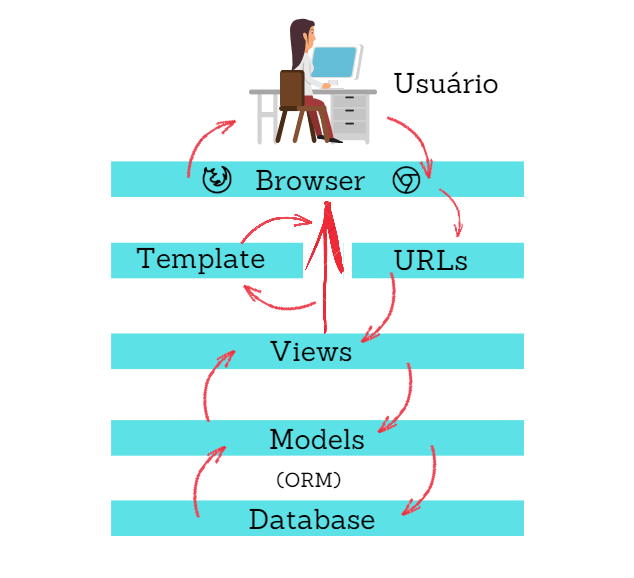
\includegraphics[width=0.85\textwidth]{Figuras/mvt-django.png}
    \caption*{Fonte: \cite{treinaweb2023mtv}}
    \label{fig:mtv}
\end{figure}

A diferença mais relevante entre os dois padrões está na forma como o roteamento de requisições é gerenciado. No MVC clássico, o \textit{Controller} é o ponto de entrada das requisições do cliente. No MTV do Django, esse papel é desempenhado pelo próprio mecanismo de roteamento de URLs do \textit{framework}, que mapeia cada endereço recebido para a \textit{View} correspondente por meio do arquivo \texttt{urls.py}, antes mesmo de qualquer lógica da aplicação ser acionada \cite{djangodocs}. A Figura~\ref{fig:mvc-vs-mtv} compara os dois padrões.

\begin{figure}[!htb]
    \centering
    \caption{Comparação entre as arquiteturas MVC e MTV}
    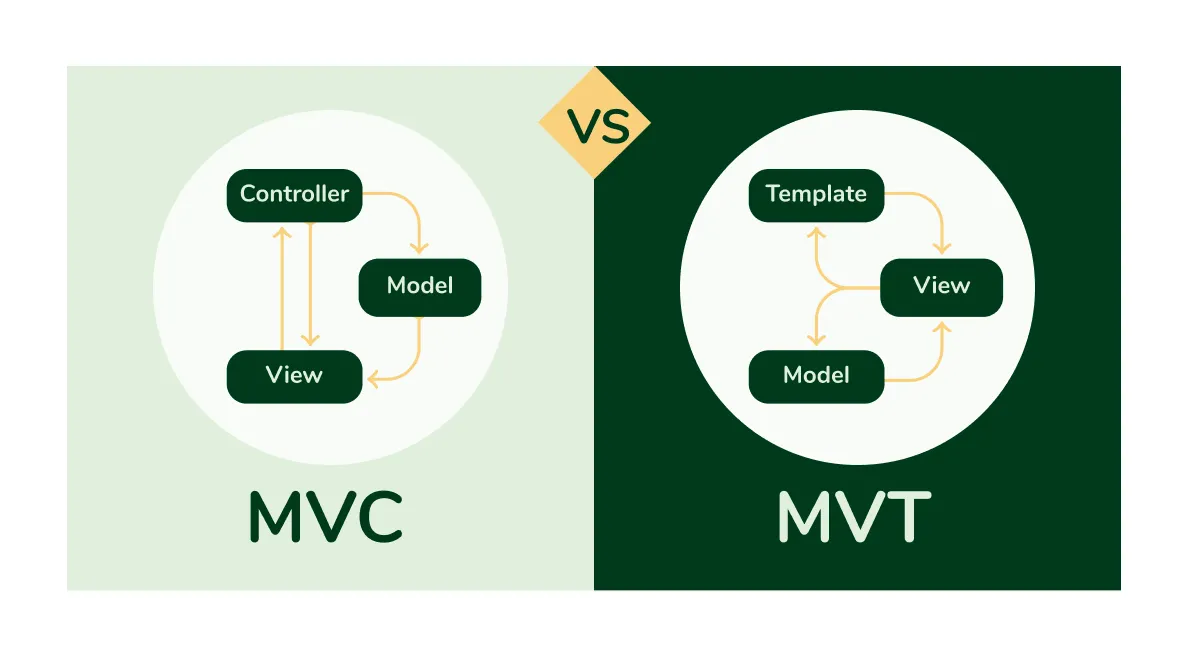
\includegraphics[width=0.85\textwidth]{Figuras/mvcVSmvt.png}
    \caption*{Fonte: \cite{djangodocs}}
    \label{fig:mvc-vs-mtv}
\end{figure}

O fluxo de uma requisição no Django, representado na Figura~\ref{fig:fluxo-mtv}, percorre essas camadas de forma sequencial: o cliente envia uma requisição HTTP, o roteador de URLs identifica a \textit{View} responsável, a \textit{View} acessa os \textit{Models} para obter ou persistir dados e, em seguida, seleciona o \textit{Template} adequado para gerar a resposta enviada de volta ao cliente \cite{silva2023mtv}.

\begin{figure}[!htb]
    \centering
    \caption{Fluxo de requisição na arquitetura MTV do Django}
    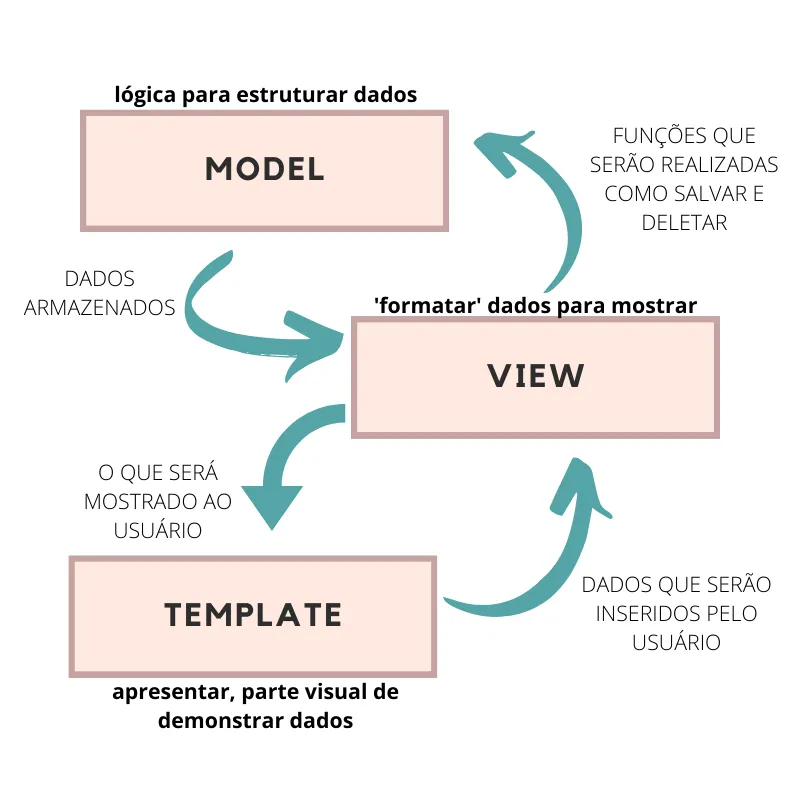
\includegraphics[width=0.85\textwidth]{Figuras/arquitetura.png}
    \caption*{Fonte: \cite{silva2023mtv}}
    \label{fig:fluxo-mtv}
\end{figure}

%-----------------------------------
\subsubsection{O Framework Django}
\label{sec:django}

O Django é um \textit{framework} web de código aberto escrito em Python. Seu conjunto de recursos inclui ORM, autenticação, roteamento de URLs, mecanismo de \textit{templates} e envio de e-mails, embora cada aplicação possa utilizar bibliotecas adicionais conforme suas necessidades \cite{djangodocs}. O \textit{framework} também segue o princípio \textit{Don't Repeat Yourself} (DRY), que orienta o reaproveitamento de código e a centralização de lógicas que, se duplicadas, aumentariam o custo de manutenção \cite{djangodocs}.

O roteamento de URLs é configurado no arquivo \texttt{urls.py}, que associa cada padrão de endereço a uma \textit{view} específica por meio da função \texttt{path()}. Quando uma requisição chega ao servidor, o \textit{framework} percorre a lista de padrões registrados até encontrar o primeiro que corresponda à URL solicitada e delega o processamento à \textit{view} associada. Esse mecanismo é independente da estrutura de diretórios da aplicação, o que permite organizar as URLs de forma legível e separada da lógica de negócio \cite{djangodocs}.

Cada \textit{model} do Django é uma classe Python que herda de \texttt{django.db.models.Model}. Cada atributo da classe representa uma coluna da tabela correspondente no banco de dados, e o tipo do campo, como \texttt{CharField}, \texttt{DateTimeField} ou \texttt{BooleanField}, determina o tipo de dado armazenado e as validações aplicadas \cite{djangodocs}. Relacionamentos entre entidades são representados por campos específicos: \texttt{ForeignKey} para associações muitos-para-um e \texttt{ManyToManyField} para associações muitos-para-muitos. O ORM traduz as operações sobre esses objetos Python em comandos SQL compatíveis com o banco de dados configurado \cite{djangodocs}.

As mudanças nos \textit{models} são controladas pelo sistema de \textit{migrations}. O comando \texttt{makemigrations} gera um arquivo descrevendo as alterações a serem aplicadas no banco; o comando \texttt{migrate} as aplica de forma incremental e rastreável, mantendo um histórico completo de todas as versões do esquema \cite{djangodocs}.

O sistema de \textit{templates} do Django utiliza a \textit{Django Template Language} (DTL), que insere dados dinâmicos nas páginas HTML por meio de variáveis e \textit{tags} de controle. Com a herança de \textit{templates}, obtida pelas \textit{tags} \texttt{\{\% extends \%\}} e \texttt{\{\% block \%\}}, um arquivo base define elementos comuns, como cabeçalho, menu e rodapé. Os demais arquivos sobrescrevem apenas os blocos específicos de cada página \cite{djangodocs}.

O Django inclui mecanismos de segurança que precisam ser habilitados e utilizados conforme a documentação. A proteção contra \textit{Cross-Site Request Forgery} (CSRF) usa um \textit{middleware} e o \textit{token} inserido pela \textit{tag} \texttt{\{\% csrf\_token \%\}} nos formulários. O sistema de \textit{templates} realiza escape automático do conteúdo dinâmico, reduzindo o risco de \textit{Cross-Site Scripting} (XSS) quando os mecanismos padrão não são desativados. Nas consultas feitas pelo ORM, os parâmetros são separados do comando SQL, o que reduz o risco de injeção; consultas SQL escritas manualmente ainda precisam seguir as práticas de segurança recomendadas \cite{djangodocs}.

%-----------------------------------
\subsubsection{Usabilidade e Interface do Usuário}
\label{sec:usab}

Usabilidade é a medida em que um produto pode ser usado por pessoas específicas para atingir objetivos específicos com eficácia, eficiência e satisfação num determinado contexto \cite{nielsen1993}. \citeonline{nielsen1993} descreve cinco atributos que compõem a usabilidade de um sistema: facilidade de aprendizado, eficiência de uso, facilidade de memorização, baixa taxa de erros e satisfação subjetiva do usuário. Um sistema com boa usabilidade permite que o usuário realize suas tarefas sem depender de treinamento extensivo nem de suporte constante.

Para orientar o projeto de interfaces, \citeonline{nielsen1994} propôs dez heurísticas de usabilidade que se tornaram referência na área: (1) visibilidade do estado do sistema, mantendo o usuário informado sobre o que está acontecendo; (2) correspondência entre o sistema e o mundo real, usando linguagem e convenções familiares ao usuário; (3) controle e liberdade do usuário, permitindo desfazer ações e sair de estados indesejados; (4) consistência e padrões, seguindo convenções da plataforma para que o usuário não precise aprender novos significados; (5) prevenção de erros, projetando para evitar que erros ocorram; (6) reconhecimento em vez de memorização, tornando objetos e opções visíveis para reduzir a carga de memória do usuário; (7) flexibilidade e eficiência de uso, permitindo que usuários experientes realizem tarefas mais rapidamente; (8) estética e design minimalista, evitando informações irrelevantes que competem com o conteúdo principal; (9) ajuda para reconhecer, diagnosticar e recuperar erros, exibindo mensagens claras sobre o que deu errado e como corrigir; e (10) ajuda e documentação, oferecendo suporte quando necessário, de forma fácil de buscar e orientada à tarefa.

Algumas dessas heurísticas têm peso particular no sistema proposto. A visibilidade do estado do sistema é importante porque o docente precisa saber, a qualquer momento, se a sua solicitação de reserva está pendente, aprovada ou rejeitada. A correspondência com o mundo real orienta o uso de termos como ``laboratório'', ``reserva'' e ``disponível'' em vez de jargões técnicos. A prevenção de erros, por sua vez, inclui mecanismos como a verificação automática de conflitos de horário antes de permitir a solicitação.

No contexto deste trabalho, usabilidade é relevante porque o sistema é destinado a docentes com familiaridade tecnológica variada. Um sistema que exija treinamento extensivo ou que gere dúvidas frequentes tende a ser abandonado, o que comprometeria o próprio objetivo de substituir o processo manual de agendamento.
%-----------------------------------
\subsubsection{Testes de Software}
\label{sec:testes}

Testes de software são atividades planejadas com o objetivo de verificar se um sistema se comporta conforme o esperado e identificar defeitos antes que o produto chegue ao usuário final. \citeonline{sommerville2018} define teste como um processo de validação e verificação que busca demonstrar que o software atende aos seus requisitos e identificar situações em que ele se comporta de forma incorreta ou inesperada. \citeonline{pressman2016} complementam essa perspectiva ao afirmar que testar é executar um programa com a intenção explícita de encontrar erros, distinguindo o processo de testes de outras atividades de garantia de qualidade por seu caráter sistematicamente verificativo: um teste bem-sucedido é aquele que revela um defeito até então desconhecido.

Os testes unitários são a forma mais elementar de teste de software e têm como foco verificar o comportamento de unidades individuais de código de forma isolada, antes de integrá-las ao restante do sistema. \citeonline{myers2011} definem teste unitário como o processo de testar subprogramas, funções ou métodos de maneira independente, de modo que, quando uma unidade falha, a localização do defeito seja imediata, sem a necessidade de investigar interações entre múltiplos componentes. \citeonline{pressman2016} acrescentam que os testes unitários devem cobrir as estruturas de controle internas de cada componente, as condições de contorno, os caminhos independentes de execução e o tratamento de erros.

No contexto de sistemas web com regras de negócio definidas, os testes unitários têm papel direto na validação da lógica da aplicação. \citeonline{sommerville2018} observa que os testes unitários são especialmente eficazes para validar componentes que implementam regras de negócio, pois permitem verificar cada condição individualmente e com precisão. À medida que as unidades validadas são combinadas, os testes de integração verificam se os componentes interagem corretamente entre si \cite{pressman2016}.

%---------------------------------
% SEÇÃO DE METODOLOGIA
%---------------------------------

\chapter{Metodologia}
\label{sec:metodologia}

Este capítulo descreveu a metodologia da pesquisa. A Seção~\ref{sec:tipopesquisa} classificou a pesquisa quanto à natureza, aos objetivos e ao procedimento técnico, e a Seção~\ref{sec:procedimentos} descreveu as etapas do trabalho.

%-----------------------------------
\subsection{Tipo de Pesquisa}
\label{sec:tipopesquisa}

Quanto à natureza, esta pesquisa foi aplicada. Sua finalidade foi produzir um artefato de software para um problema concreto identificado num contexto institucional real, não ampliar o conhecimento teórico de forma genérica. \citeonline{gil2008} distinguiu a pesquisa aplicada da pesquisa básica precisamente por esse critério: a primeira foi motivada pela necessidade de resolver problemas práticos e seus resultados tiveram aplicação imediata.

Quanto aos objetivos, a pesquisa foi descritiva. O ponto de partida foi a caracterização do processo de agendamento de espaços físicos no IFNMG -- Campus Salinas: como ele funcionava, onde falhava e o que os usuários envolvidos precisavam que mudasse. \citeonline{gil2008} definiu a pesquisa descritiva como aquela que buscava descrever as características de determinado fenômeno e estabelecer relações entre suas variáveis, sem que o pesquisador interferisse nos fatos observados.

Quanto ao procedimento técnico, a pesquisa adota o estudo de caso em combinação com pesquisa bibliográfica. O estudo de caso é adequado porque a investigação recai sobre um ambiente específico, o Campus Salinas, com histórico, atores e restrições próprios que precisam ser compreendidos antes de qualquer proposta de solução. \citeonline{yin2015} define o estudo de caso como uma investigação empírica que examina um fenômeno contemporâneo em profundidade e em seu contexto real, sendo especialmente indicado quando os limites entre o fenômeno e o contexto não são claramente separáveis. A pesquisa bibliográfica, por sua vez, dá sustentação às decisões de projeto, de modelagem e de escolha tecnológica, com base no que a literatura já consolidou sobre engenharia de software, controle de acesso e desenvolvimento web.

%-----------------------------------
\subsection{Procedimentos Metodológicos}
\label{sec:procedimentos}

Esta pesquisa foi organizada em cinco etapas: diagnóstico do problema, levantamento e análise de requisitos, modelagem do sistema, implementação e validação. As etapas foram conduzidas de forma iterativa: a cada reunião com a Direção de Ensino, os requisitos eram refinados e incorporados ao sistema em desenvolvimento. Ao final do trabalho, foram concluídas as cinco etapas: diagnóstico do problema, levantamento e análise de requisitos, modelagem, implementação e validação técnica por meio de testes automatizados.

%-----------------------------------
\subsubsection{Diagnóstico do Problema}
\label{sec:coleta}

A primeira etapa consistiu no diagnóstico do problema. Por meio de conversas semiestruturadas, interações técnicas informais e validações contínuas com a Diretora de Ensino Técnico, responsável pela gestão dos espaços físicos no campus, foram mapeados o processo atual de agendamento, suas limitações operacionais e as necessidades concretas dos usuários envolvidos, como docentes e equipe administrativa, além da consulta pública, disponível sem autenticação. As informações obtidas nessa etapa fundamentaram a especificação dos requisitos apresentada a seguir.

Os dados desta pesquisa são primários e foram coletados diretamente com a responsável pelo processo. O levantamento ocorreu de forma iterativa, por meio de conversas semiestruturadas, interações técnicas, trocas de mensagens e discussões sobre o agendamento. \citeonline{gil2008} aponta a entrevista como uma das técnicas de coleta de dados mais utilizadas nas ciências sociais por permitir que o entrevistador obtenha informações sobre fatos, opiniões, percepções e necessidades de forma direta, com abertura para explorar aspectos não previstos no roteiro inicial. Neste trabalho, essa característica foi estendida para um formato iterativo, em que o diálogo com a fonte se prolongou para além de sessões pontuais.

As interações foram conduzidas com a Diretora de Ensino Técnico do IFNMG -- Campus Salinas, responsável pela gestão dos agendamentos de espaços físicos no campus. Na fase de especificação, foram realizadas três sessões remotas: em julho de 2025, novembro de 2025 e abril de 2026.

A primeira sessão mapeou o processo atual de agendamento, incluindo a forma de solicitar reservas, os responsáveis pelo controle, os conflitos mais frequentes e as informações consultadas pelos usuários. A segunda foi dedicada à validação dos requisitos preliminares. As informações levantadas foram apresentadas de forma organizada para que a Diretora confirmasse, corrigisse ou complementasse o entendimento do pesquisador. A terceira sessão confirmou os requisitos finais e esclareceu questões surgidas durante a modelagem.

Entre essas sessões, houve comunicação técnica por mensagens e reuniões breves. Esses contatos foram usados para esclarecer dúvidas sobre o processo e validar decisões de modelagem à medida que surgiam.

Durante o desenvolvimento, foram realizadas mais três reuniões remotas. Em agosto de 2026, a planilha de horários do campus foi apresentada e os requisitos foram refinados. Em setembro de 2026, uma reunião tratou de novos refinamentos, e outra apresentou o sistema em funcionamento à Direção de Ensino.

A opção pelo formato semiestruturado permitiu seguir um roteiro comum sem limitar a discussão aos temas previstos inicialmente. O caráter iterativo foi necessário porque novas dúvidas surgiram durante a modelagem e precisaram ser confirmadas com a responsável pelo processo. Por isso, o levantamento não se limitou a uma única entrevista ou a um questionário fechado.

Como a Diretora de Ensino era a responsável pelo processo de agendamento e apresentou a necessidade que originou o sistema, ela foi adotada como principal referência institucional para o levantamento e a validação dos requisitos. Os requisitos foram discutidos, refinados e validados nas reuniões realizadas ao longo do desenvolvimento. As percepções dos docentes e dos demais usuários não foram submetidas a uma avaliação formal de usabilidade, o que constituiu uma limitação deste trabalho.

O diagnóstico mostrou que o sistema em uso exige o cadastro manual de todos os horários ocupados antes de qualquer reserva, e esse cadastro é refeito a cada semestre. Os docentes não consultam a disponibilidade nem solicitam reservas sem passar por um servidor, o que concentra todo o controle em um único ponto. Também não há registro consolidado do uso dos espaços que apoie o planejamento da administração.

Dessas limitações derivam as necessidades que orientaram os requisitos: importar a planilha de horários já produzida pelo campus, marcando automaticamente como ocupados os horários das aulas; manter essa ocupação atualizada por reimportação ou ajuste pontual, sem integração em tempo real com sistemas externos; notificar automaticamente os envolvidos no fluxo de reserva; permitir a consulta pública da ocupação; e gerar um mapa da utilização dos espaços ao longo do semestre.

%-----------------------------------
\subsubsection{Levantamento e Análise de Requisitos}
\label{sec:requisitos}

A segunda etapa foi o levantamento e a análise de requisitos. \citeonline{pressman2016} descrevem a engenharia de requisitos como um processo contínuo de identificação, análise, especificação e validação das necessidades dos envolvidos, e ressaltam que a qualidade dessa etapa determina a qualidade do que será desenvolvido depois. A especificação de requisitos foi elaborada a partir das informações coletadas nas reuniões e do referencial bibliográfico consultado, e organizada em duas categorias: requisitos funcionais e requisitos não funcionais.

Os requisitos funcionais descrevem o que o sistema deve fazer, ou seja, as funções e os serviços que ele oferece aos usuários \cite{sommerville2018}. Como o acesso é definido por perfis configuráveis (Seção~\ref{sec:rbac}), cada funcionalidade fica disponível a quem tiver a permissão correspondente, e não a um perfil fixo. A Tabela~\ref{tab:rf} apresenta os requisitos funcionais, agrupados nos módulos: ensalamento (RF01, RF02, RF13--RF16); espaços, cursos, disciplinas e turmas (RF03, RF17); usuários e perfis (RF04, RF18--RF20); agenda de reservas (RF05--RF08, RF21--RF23); notificações e comunicados (RF09, RF10, RF24); consulta pública (RF11, RF28); painel, relatórios e auditoria (RF12, RF25, RF26); configurações (RF27); e central de ajuda (RF29).

\begin{SingleSpace}
\begin{longtable}{@{}p{1.8cm}p{12cm}@{}}
	\caption{Requisitos funcionais do sistema}\label{tab:rf} \\
	\hline
	\textbf{Código} & \textbf{Descrição} \\ \hline
	\endfirsthead
	\multicolumn{2}{@{}l}{\small\textit{Continuação da Tabela~\thetable}} \\ \hline
	\textbf{Código} & \textbf{Descrição} \\ \hline
	\endhead
	\hline
	\endfoot
	RF01 & Importar a planilha de horários institucional do semestre, identificando automaticamente os espaços e os horários ocupados pelas aulas, com prévia do resultado e confirmação antes da gravação \\
	RF02 & Atualizar os horários ocupados ao longo do semestre, por reimportação da planilha ou pela manutenção das aulas no próprio sistema (RF13 a RF16) \\
	RF03 & Cadastrar e manter os espaços físicos do campus, incluindo os outros nomes pelos quais aparecem na planilha e a desativação de espaços fora de uso \\
	RF04 & Gerenciar usuários e atribuir a cada um perfil de acesso \\
	RF05 & Consultar a disponibilidade dos espaços físicos \\
	RF06 & Submeter solicitações de reserva de espaços físicos \\
	RF07 & Aprovar ou rejeitar solicitações de reserva \\
	RF08 & Cancelar reservas já aprovadas \\
	RF09 & Notificar automaticamente, no próprio sistema, os responsáveis pela análise quando uma nova solicitação de reserva for submetida \\
	RF10 & Notificar automaticamente, no próprio sistema, o solicitante sobre o resultado da análise da sua solicitação \\
	RF11 & Disponibilizar consulta pública, sem autenticação, aos horários dos espaços por sala, docente, curso ou turma, com o horário original e o calendário por data, sem expor e-mails nem a descrição das reservas \\
	RF12 & Gerar relatórios sobre a utilização dos espaços, incluindo o mapa de ocupação por dia e horário e o relatório das solicitações de reserva \\
	RF13 & Cadastrar aula recorrente, informando turma, disciplina, docentes, espaço, período de vigência, horário e duração \\
	RF14 & Alterar a recorrência de uma aula (dia, horário, duração, espaço ou docentes) a partir de uma data, sem alterar as ocorrências anteriores \\
	RF15 & Encerrar a recorrência de uma aula a partir de uma data, preservando o histórico das ocorrências anteriores \\
	RF16 & Cancelar a ocorrência de uma aula em uma data, sem alterar a recorrência, pelo administrador ou pelo docente da aula \\
	RF17 & Cadastrar e manter cursos, disciplinas e turmas \\
	RF18 & Criar perfis de acesso e definir as permissões de cada um \\
	RF19 & Importar usuários em lote por meio de arquivo CSV \\
	RF20 & Enviar ao novo usuário, por e-mail, o link para definir a senha, e permitir a recuperação de senha \\
	RF21 & Sugerir ao solicitante uma alternativa à reserva solicitada (outro espaço, data ou horário), que ele pode aceitar ou recusar \\
	RF22 & Registrar solicitação de reserva em nome de outro usuário \\
	RF23 & Acompanhar as próprias solicitações e ver a própria agenda de aulas e reservas \\
	RF24 & Publicar comunicados para todos os usuários, para os usuários de um perfil ou para usuários escolhidos \\
	RF25 & Exibir painel administrativo com as solicitações pendentes, a ocupação dos espaços e as pendências da grade (aulas sem espaço ou sem docente, conflitos de docente, choques entre aulas e reservas) \\
	RF26 & Registrar em auditoria as ações realizadas no sistema e permitir consultá-las com filtros \\
	RF27 & Configurar o servidor de envio de e-mails pela interface do sistema \\
	RF28 & Exportar o calendário público do semestre, com os filtros escolhidos, em arquivo iCalendar (.ics), para importação em aplicativos de agenda \\
	RF29 & Disponibilizar uma central de ajuda com tutoriais passo a passo de cada funcionalidade, com capturas das telas no computador e no celular, mostrando ao usuário só as funcionalidades liberadas para o seu perfil e abrindo direto na ajuda da tela de onde foi acessada \\
\end{longtable}
\end{SingleSpace}

Os requisitos não funcionais estabelecem as restrições de qualidade que o sistema precisa satisfazer \cite{sommerville2018}. Eles foram definidos a partir dos atributos de qualidade descritos pelo autor: confiabilidade e segurança (RNF01, RNF02, RNF07, RNF08, RNF09); eficiência (RNF03, RNF10, RNF11); aceitabilidade (RNF04, RNF05, RNF13); e manutenibilidade (RNF06, RNF12). \citeonline{pressman2016} reforçam que esses requisitos condicionam a arquitetura e devem ser considerados desde o início do projeto. A Tabela~\ref{tab:rnf} apresenta os requisitos não funcionais.

\begin{table}[!htb]
	\centering
	\caption{Requisitos não funcionais do sistema}
	\begin{tabular}{@{}p{1.8cm}p{12cm}@{}}
	\hline
		\textbf{Código} & \textbf{Descrição} \\ \hline
		RNF01 & Controlar o acesso com base em papéis (RBAC), restringindo cada funcionalidade ao perfil correspondente \\
		RNF02 & Proteger os dados dos usuários contra acessos indevidos: proteções contra CSRF, XSS e injeção de SQL, senha do servidor de e-mail armazenada cifrada, recuperação de senha que não revela quais e-mails estão cadastrados e encerramento das sessões do usuário quando outra pessoa altera o perfil ou o e-mail dele \\
		RNF03 & Ter tempo de resposta adequado nas consultas de disponibilidade, mesmo nos períodos de pico \\
		RNF04 & Funcionar no navegador web, sem instalar nada nos dispositivos dos usuários \\
		RNF05 & Ter usabilidade compatível com o perfil tecnológico dos docentes e consistência visual entre as telas, sem exigir treinamento extenso \\
		RNF06 & Ser manutenível, com separação clara entre as camadas de dados, lógica e apresentação \\
		RNF07 & Funcionar sem depender da infraestrutura de horários do campus, sem consultas em tempo real a sistemas externos \\
		RNF08 & Impedir reservas sobrepostas de um mesmo espaço, mesmo quando solicitações são analisadas ao mesmo tempo, por restrição de integridade no banco \\
		RNF09 & Não permitir alterar nem excluir os registros de auditoria \\
		RNF10 & Enviar os e-mails em segundo plano, com novas tentativas em caso de falha, sem atrasar a resposta ao usuário \\
		RNF11 & Exibir as notificações em tempo real, sem recarregar a página \\
		RNF12 & Ser distribuído em contêineres, para facilitar a execução em ambientes diferentes \\
		RNF13 & Adaptar as telas a computadores e celulares \\ \hline
	\end{tabular}
	\label{tab:rnf}
\end{table}

%-----------------------------------
\subsubsection{Modelagem do Sistema}
\label{sec:modelagem}

A modelagem utilizou três diagramas da UML: casos de uso, classes e sequência. Os diagramas refletem a versão implementada do sistema.

O diagrama de casos de uso (Figura~\ref{fig:casos_uso}) organiza as funcionalidades em módulos. Como os perfis do sistema são configuráveis (Seção~\ref{sec:rbac}), cada ator representa um conjunto de permissões, e não um perfil fixo: Solicitante, Analista de reservas, Gestor do ensalamento e Administrador especializam o Usuário autenticado, e o Superadministrador especializa o Administrador. O Visitante representa a consulta pública, sem autenticação.

\begin{figure}[!htb]
    \centering
    \caption{Diagrama de Casos de Uso do Sistema de Agendamento}
    \resizebox{\textwidth}{!}{% Diagrama de casos de uso do sistema de agendamento (gerado por gen_uc.py).
% Os atores representam conjuntos de permissões, e não perfis fixos.
\begin{tikzpicture}[
    font=\footnotesize,
    uc/.style={ellipse, draw, fill=white, minimum width=4.4cm, minimum height=0.8cm,
               align=center, inner xsep=-2pt, inner ysep=2.5pt},
    pkg/.style={draw, rounded corners=2pt, fill=black!4},
    pkglabel/.style={font=\scriptsize\bfseries, anchor=north west, inner sep=3pt},
    rel/.style={dashed, -{Stealth[length=2mm]}},
    rellabel/.style={font=\scriptsize\itshape, right, inner sep=2pt},
    gen/.style={-{Triangle[open, length=2.5mm, width=2.5mm]}},
    lbl/.style={anchor=north, align=center},
    hit/.style={minimum width=0.7cm, minimum height=1.3cm},
    actor/.pic={
        \draw (0,0.55) circle (0.17);
        \draw (0,0.38) -- (0,-0.1) (-0.3,0.22) -- (0.3,0.22)
              (0,-0.1) -- (-0.25,-0.5) (0,-0.1) -- (0.25,-0.5);
    },
]
\draw[thick, rounded corners=4pt] (2.6,-0.55) rectangle (13.4,20.45);
\node[font=\small\bfseries] at (8,20.05) {Sistema de Agendamento de Espaços Físicos};
\draw[pkg] (2.8499999999999996,16.0) rectangle (7.85,19.6);
\node[pkglabel] at (2.8499999999999996,19.6) {Consulta pública};
\draw[pkg] (2.8499999999999996,6.35) rectangle (7.85,15.7);
\node[pkglabel] at (2.8499999999999996,15.7) {Agenda de reservas};
\draw[pkg] (2.8499999999999996,2.45) rectangle (7.85,6.05);
\node[pkglabel] at (2.8499999999999996,6.05) {Comunicação e ajuda};
\draw[pkg] (8.15,12.55) rectangle (13.15,19.6);
\node[pkglabel] at (8.15,19.6) {Ensalamento};
\draw[pkg] (8.15,9.15) rectangle (13.15,12.25);
\node[pkglabel] at (8.15,12.25) {Cadastros};
\draw[pkg] (8.15,5.25) rectangle (13.15,8.85);
\node[pkglabel] at (8.15,8.85) {Administração do sistema};
\draw[pkg] (8.15,-0.25) rectangle (13.15,4.95);
\node[pkglabel] at (8.15,4.95) {Gestão};
\node[uc] (consultar) at (5.35,18.45) {Consultar calendário\\público};
\node[uc] (exportar) at (5.35,16.9) {Exportar calendário\\(.ics)};
\node[uc] (acompanhar) at (5.35,14.55) {Acompanhar e\\cancelar solicitações};
\node[uc] (solicitar) at (5.35,13.25) {Solicitar reserva};
\node[uc] (verificar) at (5.35,11.6) {Verificar\\disponibilidade};
\node[uc] (analisar) at (5.35,9.95) {Analisar solicitação};
\node[uc] (sugerir) at (5.35,8.55) {Sugerir alternativa};
\node[uc] (emnome) at (5.35,7.25) {Solicitar em nome\\de outro usuário};
\node[uc] (receber) at (5.35,4.9) {Receber\\notificações};
\node[uc] (ajuda) at (5.35,3.35) {Consultar central\\de ajuda};
\node[uc] (importar) at (10.65,18.45) {Importar planilha\\de horários};
\node[uc] (resolver) at (10.65,16.55) {Resolver espaços\\da planilha};
\node[uc] (aulas) at (10.65,15.0) {Manter aulas\\recorrentes};
\node[uc] (ocorrencia) at (10.65,13.45) {Cancelar ocorrência\\de aula};
\node[uc] (espacos) at (10.65,11.35) {Manter espaços};
\node[uc] (cursos) at (10.65,10.05) {Manter cursos,\\disciplinas e turmas};
\node[uc] (perfis) at (10.65,7.7) {Gerenciar perfis\\e permissões};
\node[uc] (email) at (10.65,6.15) {Configurar servidor\\de e-mail};
\node[uc] (usuarios) at (10.65,4.05) {Gerenciar usuários};
\node[uc] (painel) at (10.65,2.75) {Consultar painel\\e relatórios};
\node[uc] (auditoria) at (10.65,1.45) {Consultar auditoria};
\node[uc] (comunicado) at (10.65,0.4) {Publicar comunicado};
\draw[rel] (solicitar) -- node[rellabel] {«include»} (verificar);
\draw[rel] (analisar) -- node[rellabel] {«include»} (verificar);
\draw[rel] (sugerir) -- node[rellabel] {«extend»} (analisar);
\draw[rel] (importar) -- node[rellabel] {«include»} (resolver);
\pic at (1.2,17.675) {actor};
\node[hit] (Avis) at (1.2,17.725) {};
\node[lbl] (Lvis) at (1.2,17.125) {Visitante};
\draw (Avis) -- (consultar.west);
\draw (Avis) -- (exportar.west);
\pic at (0.6,13.9) {actor};
\node[hit] (Asol) at (0.6,13.950) {};
\node[lbl] (Lsol) at (0.6,13.350) {Solicitante};
\draw (Asol) -- (acompanhar.west);
\draw (Asol) -- (solicitar.west);
\pic at (1.6,7.5) {actor};
\node[hit] (Aana) at (1.6,7.550) {};
\node[lbl] (Lana) at (1.6,6.950) {Analista de\\reservas};
\draw (Aana) -- (analisar.west);
\draw (Aana) -- (emnome.west);
\pic at (1.2,4.125) {actor};
\node[hit] (Aaut) at (1.2,4.175) {};
\node[lbl] (Laut) at (1.2,3.575) {Usuário\\autenticado};
\draw (Aaut) -- (receber.west);
\draw (Aaut) -- (ajuda.west);
\pic at (15.0,10.65) {actor};
\node[hit] (Ages) at (15.0,10.700) {};
\node[lbl] (Lges) at (15.0,10.100) {Gestor do\\ensalamento};
\draw (Ages) -- (importar.east);
\draw (Ages) -- (aulas.east);
\draw (Ages) -- (ocorrencia.east);
\draw (Ages) -- (espacos.east);
\draw (Ages) -- (cursos.east);
\pic at (15.0,6.25) {actor};
\node[hit] (Asup) at (15.0,6.300) {};
\node[lbl] (Lsup) at (15.0,5.700) {Superadministrador};
\draw (Asup) -- (perfis.east);
\draw (Asup) -- (email.east);
\pic at (15.0,0.6000000000000001) {actor};
\node[hit] (Aadm) at (15.0,0.650) {};
\node[lbl] (Ladm) at (15.0,0.050) {Administrador};
\draw (Aadm) -- (usuarios.east);
\draw (Aadm) -- (painel.east);
\draw (Aadm) -- (auditoria.east);
\draw (Aadm) -- (comunicado.east);
\draw[gen] (Lsol.south) -- (0.6,5.34) -- (1.08,4.88);
\draw[gen] (Lana.south) -- (1.3199999999999998,4.88);
\draw[gen] (Lsup.south) -- (15.0,1.35);
\draw (Ages.east) -- (16.55,10.70) -- (16.55,-1.10);
\draw (Ladm.south) -- (15.0,-1.10);
\draw[gen] (16.55,-1.10) -- (1.2,-1.10) -- (Laut.south);
\end{tikzpicture}
}
    \caption*{Fonte: Elaborado pelo autor (2026).}
    \label{fig:casos_uso}
\end{figure}

O diagrama de classes (Figura~\ref{fig:classes}) apresenta as 18 classes do domínio, com seus atributos principais e as multiplicidades das associações. Classes de apoio, como importação, auditoria e fila de e-mails, foram omitidas para preservar a legibilidade.

O diagrama de sequência (Figura~\ref{fig:sequencia}) detalha a solicitação e a aprovação de uma reserva. Os fragmentos \textit{alt} mostram as duas verificações de conflito de horário: a primeira na solicitação e a segunda na aprovação, quando a restrição do banco de dados impede agendamentos sobrepostos (RNF08).

\begin{figure}[p]
    \centering
    \caption{Diagrama de classes do sistema}
    \resizebox{\textwidth}{!}{% Diagrama de classes do domínio do sistema de agendamento (página em pé).
% Fonte: models.py das apps accounts, schedule, bookings e notices.
% Classes de apoio (importação, auditoria, fila de e-mails) foram omitidas.
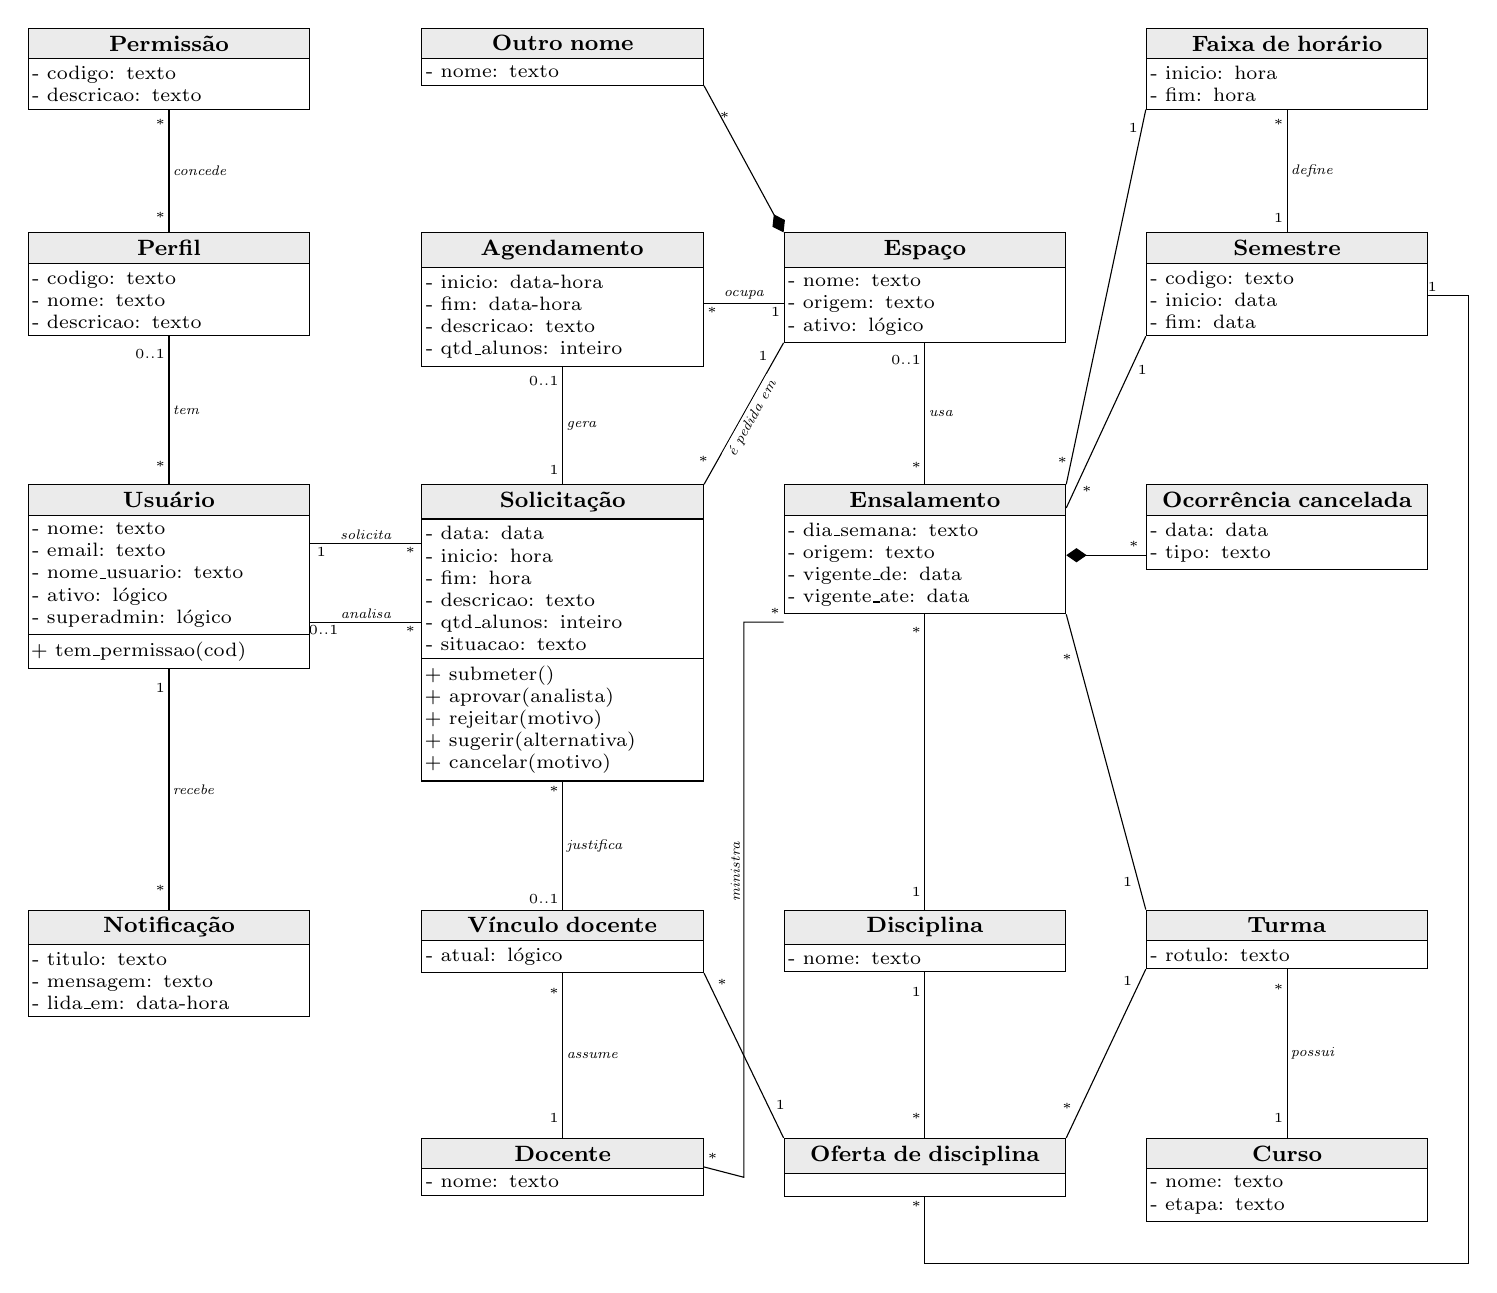
\begin{tikzpicture}[
    font=\scriptsize,
    cls/.style={draw, rectangle split, rectangle split parts=3,
                text width=3.4cm, align=left, anchor=north, inner sep=2.5pt,
                rectangle split part fill={black!8,white,white}},
    cls2/.style={draw, rectangle split, rectangle split parts=2,
                text width=3.4cm, align=left, anchor=north, inner sep=2.5pt,
                rectangle split part fill={black!8,white}},
    m/.style={font=\tiny, inner sep=1.2pt},
    rl/.style={font=\tiny\itshape, inner sep=1.2pt, fill=white},
    comp/.style={{Diamond[length=2.6mm, width=1.8mm]}-},
]
\newcommand{\cname}[1]{\centering\textbf{\footnotesize #1}\par}
\def\ca{1.85}\def\cb{6.85}\def\cc{11.45}\def\cd{16.05}
\def\ra{21.0}\def\rb{18.4}\def\rc{15.2}\def\rd{9.8}\def\re{6.9}

% ---------------- coluna 1: acesso ----------------
\node[cls2] (permissao) at (\ca,\ra) {\cname{Permissão}
  \nodepart{second} - codigo: texto\\- descricao: texto};
\node[cls2] (perfil) at (\ca,\rb) {\cname{Perfil}
  \nodepart{second} - codigo: texto\\- nome: texto\\- descricao: texto};
\node[cls] (usuario) at (\ca,\rc) {\cname{Usuário}
  \nodepart{second} - nome: texto\\- email: texto\\- nome\_usuario: texto\\- ativo: lógico\\- superadmin: lógico
  \nodepart{third} + tem\_permissao(cod)};
\node[cls2] (notificacao) at (\ca,\rd) {\cname{Notificação}
  \nodepart{second} - titulo: texto\\- mensagem: texto\\- lida\_em: data-hora};

% ---------------- coluna 2: agenda ----------------
\node[cls2] (outronome) at (\cb,\ra) {\cname{Outro nome}
  \nodepart{second} - nome: texto};
\node[cls2] (agendamento) at (\cb,\rb) {\cname{Agendamento}
  \nodepart{second} - inicio: data-hora\\- fim: data-hora\\- descricao: texto\\- qtd\_alunos: inteiro};
\node[cls] (solicitacao) at (\cb,\rc) {\cname{Solicitação}
  \nodepart{second} - data: data\\- inicio: hora\\- fim: hora\\- descricao: texto\\- qtd\_alunos: inteiro\\- situacao: texto
  \nodepart{third} + submeter()\\+ aprovar(analista)\\+ rejeitar(motivo)\\+ sugerir(alternativa)\\+ cancelar(motivo)};
\node[cls2] (vinculo) at (\cb,\rd) {\cname{Vínculo docente}
  \nodepart{second} - atual: lógico};
\node[cls2] (docente) at (\cb,\re) {\cname{Docente}
  \nodepart{second} - nome: texto};

% ---------------- coluna 3: espaços e grade ----------------
\node[cls2] (espaco) at (\cc,\rb) {\cname{Espaço}
  \nodepart{second} - nome: texto\\- origem: texto\\- ativo: lógico};
\node[cls2] (ensalamento) at (\cc,\rc) {\cname{Ensalamento}
  \nodepart{second} - dia\_semana: texto\\- origem: texto\\- vigente\_de: data\\- vigente\_ate: data};
\node[cls2] (disciplina) at (\cc,\rd) {\cname{Disciplina}
  \nodepart{second} - nome: texto};
\node[cls2] (oferta) at (\cc,\re) {\cname{Oferta de disciplina}
  \nodepart{second} \vphantom{x}};

% ---------------- coluna 4 ----------------
\node[cls2] (faixa) at (\cd,\ra) {\cname{Faixa de horário}
  \nodepart{second} - inicio: hora\\- fim: hora};
\node[cls2] (semestre) at (\cd,\rb) {\cname{Semestre}
  \nodepart{second} - codigo: texto\\- inicio: data\\- fim: data};
\node[cls2] (ocorrencia) at (\cd,\rc) {\cname{Ocorrência cancelada}
  \nodepart{second} - data: data\\- tipo: texto};
\node[cls2] (turma) at (\cd,\rd) {\cname{Turma}
  \nodepart{second} - rotulo: texto};
\node[cls2] (curso) at (\cd,\re) {\cname{Curso}
  \nodepart{second} - nome: texto\\- etapa: texto};

% ================= associações =================
% --- acesso (verticais na coluna 1)
\draw (perfil.north) -- node[rl, right] {concede} (permissao.south)
      node[m, pos=0.12, left] {*} node[m, pos=0.88, left] {*};
\draw (usuario.north) -- node[rl, right] {tem} (perfil.south)
      node[m, pos=0.12, left] {*} node[m, pos=0.88, left] {0..1};
\draw (usuario.south) -- node[rl, right] {recebe} (notificacao.north)
      node[m, pos=0.08, left] {1} node[m, pos=0.92, left] {*};

% --- usuário e solicitação (horizontais)
\path (usuario.north east) ++(0,-0.75) coordinate (s1);
\path (usuario.north east) ++(0,-1.75) coordinate (s2);
\draw (s1) -- node[rl, above] {solicita} (solicitacao.west |- s1)
      node[m, pos=0.1, below] {1} node[m, pos=0.9, below] {*};
\draw (s2) -- node[rl, above] {analisa} (solicitacao.west |- s2)
      node[m, pos=0.12, below] {0..1} node[m, pos=0.9, below] {*};

% --- agenda (verticais na coluna 2)
\draw (solicitacao.north) -- node[rl, right] {gera} (agendamento.south)
      node[m, pos=0.12, left] {1} node[m, pos=0.88, left] {0..1};
\draw (solicitacao.south) -- node[rl, right] {justifica} (vinculo.north)
      node[m, pos=0.08, left] {*} node[m, pos=0.92, left] {0..1};
\draw (docente.north) -- node[rl, right] {assume} (vinculo.south)
      node[m, pos=0.12, left] {1} node[m, pos=0.88, left] {*};

% --- espaço
\path (agendamento.north east) ++(0,-0.9) coordinate (a1);
\draw (a1) -- node[rl, above] {ocupa} (espaco.west |- a1)
      node[m, pos=0.1, below] {*} node[m, pos=0.9, below] {1};
\draw (solicitacao.north east) -- node[rl, sloped, below] {é pedida em} (espaco.south west)
      node[m, pos=0.1, above left] {*} node[m, pos=0.85, above left] {1};
\draw[comp] (espaco.north west) -- (outronome.south east)
      node[m, pos=0.85, below right] {*};

% --- ensalamento
\draw (ensalamento.north) -- node[rl, right] {usa} (espaco.south)
      node[m, pos=0.12, left] {*} node[m, pos=0.88, left] {0..1};
\draw (ensalamento.south) -- (disciplina.north)
      node[m, pos=0.06, left] {*} node[m, pos=0.94, left] {1};
\path (ensalamento.north east) ++(0,-0.9) coordinate (e1);
\draw[comp] (e1) -- (ocorrencia.west |- e1)
      node[m, pos=0.85, above] {*};
\draw ([yshift=-3mm]ensalamento.north east) -- (semestre.south west)
      node[m, pos=0.15, below right] {*} node[m, pos=0.85, below right] {1};
\draw (ensalamento.north east) -- (faixa.south west)
      node[m, pos=0.06, left] {*} node[m, pos=0.95, left] {1};
\draw (ensalamento.south east) -- (turma.north west)
      node[m, pos=0.12, below left] {*} node[m, pos=0.88, below left] {1};
\draw (docente.east) -- (\cb+2.3,\re-0.5) -- node[rl, sloped, above, pos=0.55] {ministra} (\cb+2.3,\rc-1.75)
      -- (ensalamento.south west |- 0,\rc-1.75);
\node[m, above right] at (docente.east) {*};
\node[m, above left] at (ensalamento.south west |- 0,\rc-1.75) {*};

% --- grade
\draw (semestre.north) -- node[rl, right] {define} (faixa.south)
      node[m, pos=0.12, left] {1} node[m, pos=0.88, left] {*};
\draw (vinculo.south east) -- (oferta.north west)
      node[m, pos=0.12, above right] {*} node[m, pos=0.85, above right] {1};
\draw (oferta.north) -- (disciplina.south)
      node[m, pos=0.12, left] {*} node[m, pos=0.88, left] {1};
\draw (oferta.north east) -- (turma.south west)
      node[m, pos=0.12, above left] {*} node[m, pos=0.88, above left] {1};
\draw (curso.north) -- node[rl, right] {possui} (turma.south)
      node[m, pos=0.12, left] {1} node[m, pos=0.88, left] {*};
\draw (oferta.south) -- (\cc,\re-1.6) -- (\cd+2.3,\re-1.6) -- (\cd+2.3,\rb-0.8) -- (semestre.east |- 0,\rb-0.8)
      node[m, pos=0.9, above] {1};
\node[m, below left] at (oferta.south) {*};
\end{tikzpicture}
}
    \caption*{Fonte: Elaborado pelo autor (2026).}
    \label{fig:classes}
\end{figure}

\begin{figure}[p]
    \centering
    \caption{Diagrama de sequência da solicitação e aprovação de reserva}
    \resizebox{\textwidth}{!}{% Diagrama de sequência: solicitar e aprovar uma reserva.
% Fonte: bookings/models.py (submit, approve, Booking.objects.book) e notices/events.py (announce).
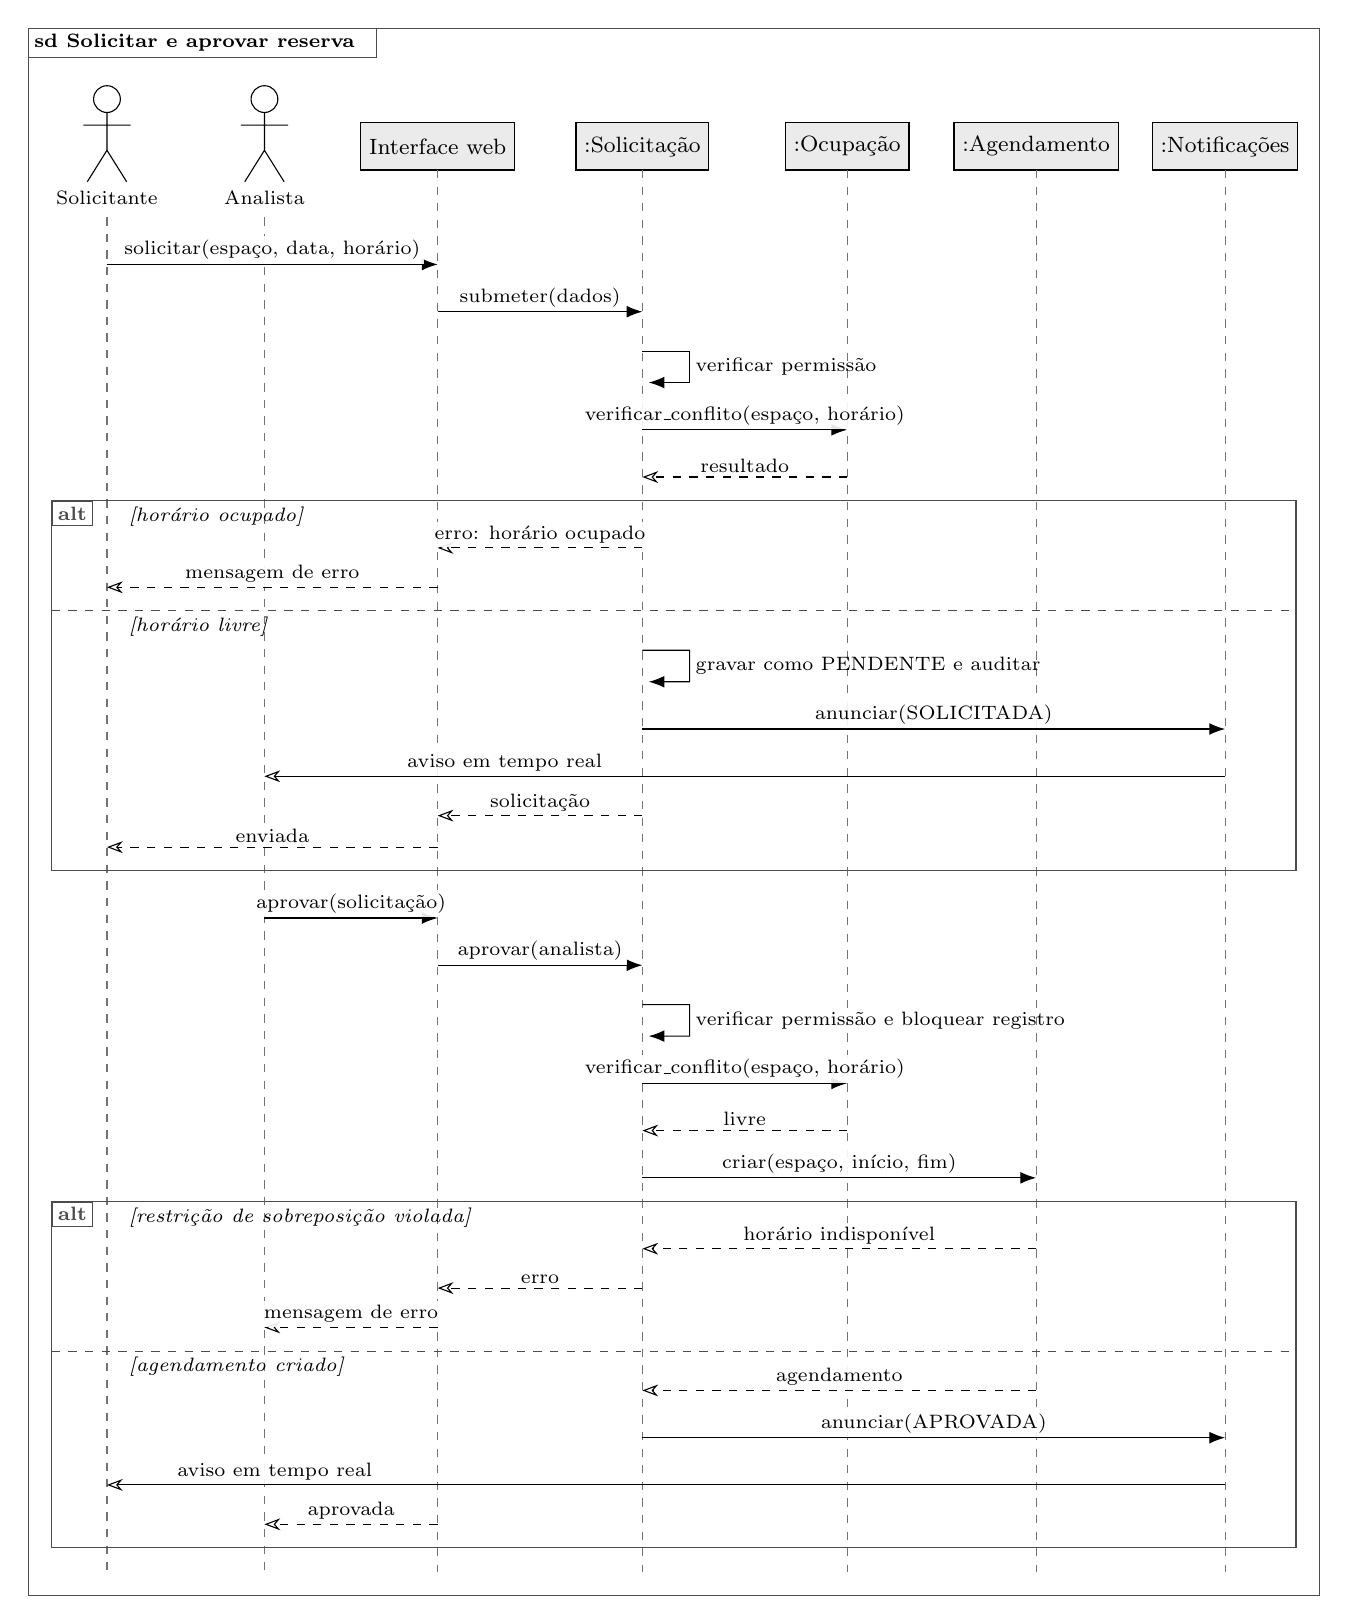
\begin{tikzpicture}[
    font=\scriptsize,
    obj/.style={draw, fill=black!8, minimum height=0.6cm, inner sep=3pt, font=\footnotesize},
    life/.style={dashed, black!55},
    call/.style={-{Latex[length=2mm]}},
    ret/.style={dashed, -{Stealth[open, length=2mm]}},
    async/.style={-{Stealth[open, length=2mm]}},
    lab/.style={above, inner sep=1.5pt, fill=white, fill opacity=0.9, text opacity=1},
    frag/.style={draw, black!70},
    guard/.style={font=\scriptsize\itshape, anchor=north west, inner sep=2pt},
    actor/.pic={
        \draw (0,0.55) circle (0.17);
        \draw (0,0.38) -- (0,-0.1) (-0.3,0.22) -- (0.3,0.22)
              (0,-0.1) -- (-0.25,-0.5) (0,-0.1) -- (0.25,-0.5);
    },
]
\def\xs{0.8}\def\xa{2.8}\def\xi{5.0}\def\xq{7.6}\def\xo{10.2}\def\xg{12.6}\def\xn{15.0}
\def\ytop{0}\def\ybot{-17.6}

% ---------- quadro sd ----------
\draw[frag] (-0.2,2.0) rectangle (16.2,\ybot-0.3);
\node[anchor=north west, inner sep=2pt, font=\scriptsize\bfseries] (sd) at (-0.2,2.0) {sd Solicitar e aprovar reserva};
\draw[frag] (sd.south west) -| ([xshift=2mm]sd.east) -- ([xshift=2mm]sd.north east);

% ---------- participantes ----------
\pic at (\xs,0.55) {actor}; \node at (\xs,-0.15) {Solicitante};
\pic at (\xa,0.55) {actor}; \node at (\xa,-0.15) {Analista};
\node[obj] at (\xi,0.5) {Interface web};
\node[obj] at (\xq,0.5) {:Solicitação};
\node[obj] at (\xo,0.5) {:Ocupação};
\node[obj] at (\xg,0.5) {:Agendamento};
\node[obj] at (\xn,0.5) {:Notificações};
\foreach \x/\y in {\xs/-0.4,\xa/-0.4,\xi/0.2,\xq/0.2,\xo/0.2,\xg/0.2,\xn/0.2}
    \draw[life] (\x,\y) -- (\x,\ybot);

% ================= 1. solicitação =================
\draw[call] (\xs,-1.0) -- node[lab] {solicitar(espaço, data, horário)} (\xi,-1.0);
\draw[call] (\xi,-1.6) -- node[lab] {submeter(dados)} (\xq,-1.6);
\draw[call] (\xq,-2.1) -- ++(0.6,0) -- ++(0,-0.4) node[right, midway, inner sep=2pt] {verificar permissão} -- (\xq+0.08,-2.5);
\draw[call] (\xq,-3.1) -- node[lab] {verificar\_conflito(espaço, horário)} (\xo,-3.1);
\draw[ret]  (\xo,-3.7) -- node[lab] {resultado} (\xq,-3.7);

% alt: conflito na solicitação
\draw[frag] (0.1,-4.0) rectangle (15.9,-8.7);
\node[draw, frag, fill=white, anchor=north west, inner sep=2pt, font=\scriptsize\bfseries] at (0.1,-4.0) {alt};
\node[guard] at (1.0,-4.0) {[horário ocupado]};
\draw[ret] (\xq,-4.6) -- node[lab] {erro: horário ocupado} (\xi,-4.6);
\draw[ret] (\xi,-5.1) -- node[lab] {mensagem de erro} (\xs,-5.1);
\draw[frag, dashed] (0.1,-5.4) -- (15.9,-5.4);
\node[guard] at (1.0,-5.4) {[horário livre]};
\draw[call] (\xq,-5.9) -- ++(0.6,0) -- ++(0,-0.4) node[right, midway, inner sep=2pt] {gravar como PENDENTE e auditar} -- (\xq+0.08,-6.3);
\draw[call] (\xq,-6.9) -- node[lab] {anunciar(SOLICITADA)} (\xn,-6.9);
\draw[async] (\xn,-7.5) -- node[lab, pos=0.75] {aviso em tempo real} (\xa,-7.5);
\draw[ret] (\xq,-8.0) -- node[lab] {solicitação} (\xi,-8.0);
\draw[ret] (\xi,-8.4) -- node[lab] {enviada} (\xs,-8.4);

% ================= 2. análise =================
\draw[call] (\xa,-9.3) -- node[lab] {aprovar(solicitação)} (\xi,-9.3);
\draw[call] (\xi,-9.9) -- node[lab] {aprovar(analista)} (\xq,-9.9);
\draw[call] (\xq,-10.4) -- ++(0.6,0) -- ++(0,-0.4) node[right, midway, inner sep=2pt] {verificar permissão e bloquear registro} -- (\xq+0.08,-10.8);
\draw[call] (\xq,-11.4) -- node[lab] {verificar\_conflito(espaço, horário)} (\xo,-11.4);
\draw[ret]  (\xo,-12.0) -- node[lab] {livre} (\xq,-12.0);
\draw[call] (\xq,-12.6) -- node[lab] {criar(espaço, início, fim)} (\xg,-12.6);

% alt: restrição do banco
\draw[frag] (0.1,-12.9) rectangle (15.9,-17.3);
\node[draw, frag, fill=white, anchor=north west, inner sep=2pt, font=\scriptsize\bfseries] at (0.1,-12.9) {alt};
\node[guard] at (1.0,-12.9) {[restrição de sobreposição violada]};
\draw[ret] (\xg,-13.5) -- node[lab] {horário indisponível} (\xq,-13.5);
\draw[ret] (\xq,-14.0) -- node[lab] {erro} (\xi,-14.0);
\draw[ret] (\xi,-14.5) -- node[lab] {mensagem de erro} (\xa,-14.5);
\draw[frag, dashed] (0.1,-14.8) -- (15.9,-14.8);
\node[guard] at (1.0,-14.8) {[agendamento criado]};
\draw[ret] (\xg,-15.3) -- node[lab] {agendamento} (\xq,-15.3);
\draw[call] (\xq,-15.9) -- node[lab] {anunciar(APROVADA)} (\xn,-15.9);
\draw[async] (\xn,-16.5) -- node[lab, pos=0.85] {aviso em tempo real} (\xs,-16.5);
\draw[ret] (\xi,-17.0) -- node[lab] {aprovada} (\xa,-17.0);
\end{tikzpicture}
}
    \caption*{Fonte: Elaborado pelo autor (2026).}
    \label{fig:sequencia}
\end{figure}

%-----------------------------------
\subsubsection{Implementação}
\label{sec:implementacao}

A quarta etapa foi a implementação. O IFAgenda foi desenvolvido como uma aplicação web, com as tecnologias e a arquitetura descritas a seguir, e constituiu uma versão funcional, executada em ambiente local e distribuída em contêineres.

A implementação utiliza Python e o \textit{framework} Django, cujo padrão arquitetural MTV e funcionamento estão descritos nas Seções~\ref{sec:mvc_mtv} e~\ref{sec:django}. O \textit{framework} fornece o ORM, o sistema de autenticação, o roteamento e o mecanismo de \textit{templates} utilizados no projeto. A separação entre dados, lógica e apresentação também organiza o código e concentra as regras de reserva em componentes próprios.

A Tabela~\ref{tab:funcionalidades} resume as funcionalidades do sistema, agrupadas pelos mesmos módulos dos requisitos funcionais.

\begin{table}[!htb]
	\centering
	\caption{Funcionalidades do sistema por módulo}
	\renewcommand{\arraystretch}{1.25}
	\newcommand{\fitem}[1]{\par\hangindent=1em\hangafter=1\noindent\makebox[1em][l]{\textbullet}#1}
	\begin{tabular}{@{}>{\raggedright\arraybackslash}p{4.0cm}>{\raggedright\arraybackslash}p{9.8cm}@{}}
	\hline
		\textbf{Módulo} & \textbf{Funcionalidades principais} \\ \hline
		Ensalamento & \fitem{Importação da planilha de horários, com prévia e confirmação}\fitem{Associação dos espaços da planilha aos já cadastrados}\fitem{Aulas recorrentes: alteração, encerramento e cancelamento de ocorrências} \\ \arrayrulecolor{black!25}\hline\arrayrulecolor{black}
		Espaços, cursos, disciplinas e turmas & \fitem{Cadastro e manutenção} \\ \arrayrulecolor{black!25}\hline\arrayrulecolor{black}
		Usuários e perfis & \fitem{Cadastro individual ou em lote (CSV)}\fitem{Definição e recuperação de senha}\fitem{Perfis com permissões definidas pelo superadministrador} \\ \arrayrulecolor{black!25}\hline\arrayrulecolor{black}
		Agenda de reservas & \fitem{Solicitação, inclusive em nome de outro usuário}\fitem{Análise: aprovação, rejeição ou sugestão de alternativa}\fitem{Acompanhamento das próprias solicitações} \\ \arrayrulecolor{black!25}\hline\arrayrulecolor{black}
		Notificações e comunicados & \fitem{Avisos em tempo real}\fitem{Comunicados para todos, para um perfil ou para usuários escolhidos} \\ \arrayrulecolor{black!25}\hline\arrayrulecolor{black}
		Consulta pública & \fitem{Calendário por data, com filtros por sala, docente, curso e turma}\fitem{Horário original da planilha}\fitem{Exportação do calendário (.ics)} \\ \arrayrulecolor{black!25}\hline\arrayrulecolor{black}
		Painel, relatórios e auditoria & \fitem{Painel de pendências e solicitações}\fitem{Mapa de ocupação por dia e horário}\fitem{Relatório de solicitações}\fitem{Registro das ações, sem alteração ou exclusão} \\ \arrayrulecolor{black!25}\hline\arrayrulecolor{black}
		Configurações & \fitem{Servidor de envio de e-mails configurado pela interface} \\ \arrayrulecolor{black!25}\hline\arrayrulecolor{black}
		Central de ajuda & \fitem{Tutoriais por tela, filtrados pelas permissões do usuário} \\ \hline
	\end{tabular}
	\label{tab:funcionalidades}
\end{table}

Para a camada de dados, foi utilizado o PostgreSQL como sistema gerenciador de banco de dados relacional. O SQLite foi mantido como alternativa adequada para desenvolvimento local, mas o PostgreSQL atende melhor ao cenário de execução definido, que envolve acessos simultâneos, transações e restrições de integridade para impedir reservas sobrepostas. O Django oferece suporte ao PostgreSQL por meio do ORM e das transações do banco \cite{djangodocs}. No projeto, o acesso aos dados é feito pelo ORM, enquanto as restrições de integridade são mantidas no esquema relacional.

A camada de apresentação foi construída com os \textit{templates} do Django combinados ao Tailwind CSS. Essa escolha agiliza o desenvolvimento da interface, mantém a consistência visual entre as telas e reduz o custo de manutenção, permitindo ajustes visuais sem alteração nas \textit{views} ou nos \textit{models}.

Para a autenticação dos usuários, foi utilizada a biblioteca \textit{django-allauth}, escolhida por fornecer prontos os fluxos de registro, login, recuperação de senha e gerenciamento de sessões \cite{pennersr2024}. O controle de acesso descrito na Seção~\ref{sec:rbac} foi implementado com perfis configuráveis. Cada permissão corresponde a uma ação sobre um recurso do sistema, como solicitar uma reserva ou editar um espaço, e o sistema define 47 permissões, distribuídas em 13 módulos. Um perfil é um conjunto dessas permissões, montado pelo superadministrador. Os perfis Administrador e Docente vêm na carga inicial apenas como exemplo e podem ser alterados. Outras categorias, como os técnicos administrativos, recebem um perfil com as permissões de que precisam. A verificação ocorre sempre no servidor, e a consulta pública dispensa autenticação.

As notificações automáticas são exibidas no próprio sistema, em um ícone no cabeçalho que se atualiza em tempo real, sem recarregar a página (RNF11). Ao receber uma solicitação de reserva, o sistema notifica os responsáveis pela análise; após a decisão, o solicitante recebe o resultado (RF09 e RF10). O e-mail é usado apenas para a definição e a recuperação de senha, com o servidor de envio configurado pela interface (RF27) e as mensagens enviadas em segundo plano (RNF10) \cite{djangodocs}.

As notificações em tempo real foram implementadas com o Django Channels, extensão que permite ao Django manter conexões WebSocket com o navegador \cite{channelsdocs}. Tarefas demoradas, como a importação da planilha e o envio de e-mails, são executadas por um processo próprio em segundo plano. Esse processo lê uma fila registrada no banco e repete o envio em caso de falha. A aplicação, o banco de dados e o processo de tarefas são distribuídos em contêineres orquestrados pelo Docker Compose \cite{dockerdocs}.

O presente trabalho limita-se ao desenvolvimento de uma versão funcional do sistema para execução em ambiente local, acessível por navegador. A hospedagem e a implantação em infraestrutura institucional não fazem parte do escopo.
%-----------------------------------
\subsubsection{Validação}
\label{sec:validacao}

A validação realizada neste trabalho ocorreu em duas frentes. A primeira correspondeu à validação do alinhamento da solução ao processo institucional, conduzida com a Diretora de Ensino, principal interessada e responsável pelos agendamentos. A segunda foi exclusivamente técnica e consistiu em testes automatizados, unitários e de integração, conforme os conceitos da Seção~\ref{sec:testes}. Os testes unitários verificaram regras e componentes de forma isolada. Os testes de integração verificaram o comportamento conjunto entre as camadas da aplicação, o banco de dados e os fluxos acessados pelos usuários.

Os testes são escritos com o \textit{framework} de testes do Django. Cada caso é executado sobre um banco de dados temporário, separado dos dados utilizados durante o desenvolvimento \cite{djangodocs}. Esse procedimento permite preparar os dados necessários para cada cenário e verificar as alterações realizadas sem modificar a base utilizada pela aplicação. A versão desenvolvida conta com mais de 1.700 casos de teste, distribuídos entre os módulos e regras de negócio do sistema.

Entre as situações verificadas estiveram o bloqueio de reservas sobrepostas, inclusive quando solicitações foram analisadas simultaneamente; a aplicação das permissões conforme o perfil do usuário; a importação e a reimportação da planilha de horários; as alterações em aulas recorrentes; o envio de notificações; a consulta pública sem exposição de dados pessoais; e a imutabilidade dos registros de auditoria. A Tabela~\ref{tab:testes} relacionou essas verificações aos requisitos correspondentes. Para a validação técnica, foi adotado como critério a execução de todos os testes automatizados sem falhas. Não foram realizados testes formais de usabilidade com usuários finais. Portanto, os testes automatizados avaliaram o funcionamento técnico do sistema, enquanto a adequação aos requisitos institucionais foi analisada nas reuniões com a Diretora de Ensino.

\begin{table}[!htb]
	\centering
	\caption{Regras de negócio verificadas pelos testes}
	\begin{tabular}{@{}>{\raggedright\arraybackslash}p{9.8cm}>{\raggedright\arraybackslash}p{4.0cm}@{}}
	\hline
		\textbf{Regra verificada} & \textbf{Requisitos} \\ \hline
		Bloqueio de reservas sobrepostas, inclusive em análises simultâneas & RF06, RF07, RNF08 \\
		Acesso a cada funcionalidade conforme as permissões do perfil & RF18, RNF01 \\
		Importação e reimportação da planilha de horários & RF01, RF02 \\
		Alteração, encerramento e cancelamento de aulas recorrentes & RF14--RF16 \\
		Envio das notificações ao solicitante e aos responsáveis & RF09, RF10 \\
		Consulta pública sem exposição de dados pessoais & RF11 \\
		Imutabilidade dos registros de auditoria & RF26, RNF09 \\ \hline
	\end{tabular}
	\label{tab:testes}
\end{table}

%---------------------------------
% SEÇÃO DE CRONOGRAMA
%---------------------------------
\needspace{9\baselineskip}

\chapter{Resultados} 
\label{cap4_resultados} 

Este capítulo apresentou os resultados obtidos com o desenvolvimento do \textit{IFAgenda}, sistema web para gerenciamento de reservas de espaços físicos no IFNMG -- Campus Salinas. Os resultados foram organizados em três aspectos: a solução implementada, o atendimento às necessidades identificadas e a validação técnica realizada.

\section{Sistema Desenvolvido}
\label{sec:resultado-sistema}

O IFAgenda constituiu uma aplicação web funcional, executada em ambiente local e acessível por navegador. A solução foi implementada em Python com o \textit{framework} Django, utilizando PostgreSQL como sistema gerenciador de banco de dados e Docker Compose para a distribuição dos componentes em contêineres. A interface foi construída com \textit{templates} do Django e Tailwind CSS.

A aplicação reuniu os módulos necessários à gestão dos espaços e das reservas. O módulo de ensalamento permitiu importar a planilha de horários do campus, revisar os dados antes da confirmação, associar os espaços da planilha aos espaços cadastrados e administrar aulas recorrentes. Os módulos de cadastro mantiveram espaços, cursos, disciplinas, turmas, usuários e perfis.

O fluxo de reservas permitiu que o usuário consultasse a disponibilidade, solicitasse uma reserva e acompanhasse suas solicitações. Os responsáveis puderam aprovar ou rejeitar pedidos e sugerir alternativas de espaço, data ou horário. A solução também ofereceu consulta pública do calendário, notificações internas em tempo real, comunicados, painel administrativo, mapa de ocupação, relatórios, exportação em formato iCalendar, auditoria das ações e central de ajuda.

\section{Atendimento às Necessidades Identificadas}
\label{sec:resultado-necessidades}

O IFAgenda atendeu às principais limitações observadas no diagnóstico. A importação da planilha reduziu o cadastro manual dos horários ocupados e permitiu que a ocupação das aulas fosse refletida no calendário do sistema. A consulta pública permitiu visualizar a ocupação sem intermediação, enquanto o fluxo de aprovação manteve o controle administrativo sobre as reservas extraordinárias.

O controle de acesso baseado em papéis restringiu as funcionalidades conforme as permissões de cada perfil. A solução definiu 47 permissões distribuídas em 13 módulos, possibilitando que os perfis fossem configurados pelo superadministrador. A restrição de integridade no banco de dados impediu reservas sobrepostas do mesmo espaço, inclusive quando solicitações foram analisadas simultaneamente.

O IFAgenda também registrou as ações realizadas em auditoria, manteve o histórico das solicitações e forneceu informações para o acompanhamento da utilização dos espaços. Dessa forma, além de organizar o processo de reserva, a aplicação ofereceu dados que puderam apoiar o planejamento da ocupação dos laboratórios e das salas especiais.

\section{Validação Técnica}
\label{sec:resultado-validacao}

A validação foi realizada com testes unitários e de integração utilizando o \textit{framework} de testes do Django. Os casos foram executados em banco de dados temporário, isolado dos dados de desenvolvimento. A versão desenvolvida contou com mais de 1.700 casos de teste distribuídos entre os módulos e as regras de negócio do sistema.

Foram verificados, entre outros aspectos, o bloqueio de reservas sobrepostas, a aplicação das permissões conforme o perfil, a importação e a reimportação da planilha, o tratamento de aulas recorrentes, o envio de notificações, a consulta pública sem exposição de dados pessoais e a imutabilidade dos registros de auditoria. A validação institucional foi realizada em reuniões com a Diretora de Ensino Técnico, que acompanhou o refinamento dos requisitos e a apresentação do sistema.

Os resultados demonstram que foi possível desenvolver uma versão funcional alinhada ao processo institucional levantado. Entretanto, não foram realizados testes formais de usabilidade com os usuários finais, e a implantação em infraestrutura institucional não fez parte do escopo. Essas limitações devem ser consideradas na interpretação dos resultados e no planejamento de evoluções futuras.
\chapter{Conclusão} 
\label{cap5_conclusao} 

Este trabalho teve como objetivo desenvolver o \textit{IFAgenda}, um sistema web para o gerenciamento de reservas de espaços físicos no IFNMG -- Campus Salinas. O problema foi investigado a partir das dificuldades do processo existente, que exigia o cadastro manual dos horários ocupados, dependia da intermediação de servidores e não mantinha um registro consolidado da utilização dos espaços.

O objetivo geral foi alcançado com o desenvolvimento de uma versão funcional da aplicação. O IFAgenda permitiu importar a planilha de horários, consultar a disponibilidade, solicitar e analisar reservas, enviar notificações, acompanhar a ocupação dos espaços e registrar as ações realizadas. Também foram implementados mecanismos de controle de acesso, consulta pública, relatórios, auditoria e central de ajuda.

Os objetivos específicos também foram contemplados. O processo atual e as necessidades dos usuários foram levantados com a Direção de Ensino Técnico; os requisitos funcionais e não funcionais foram especificados; a aplicação foi implementada com Python, Django, PostgreSQL, Tailwind CSS e Docker Compose; e o funcionamento técnico foi verificado por testes unitários e de integração. A solução conta com mais de 1.700 casos de teste distribuídos entre os módulos e as regras de negócio.

Como contribuição, o sistema organizou em uma única aplicação o ensalamento, a consulta de disponibilidade e o fluxo de reservas. A importação da planilha reduziu o trabalho manual, enquanto o controle de conflitos e o registro de auditoria aumentaram a confiabilidade do processo. A consulta pública e os relatórios também puderam apoiar a administração na visualização e no planejamento da ocupação dos espaços.

O trabalho possuiu duas limitações principais. A primeira foi que a versão desenvolvida foi executada em ambiente local, não incluindo a hospedagem e a implantação na infraestrutura institucional. A segunda foi a ausência de uma avaliação formal de usabilidade com docentes e demais usuários finais. Assim, a validação realizada demonstrou o funcionamento técnico e o alinhamento com os requisitos discutidos com a Direção de Ensino, mas não permitiu concluir sobre a experiência de uso de todos os públicos do sistema.

Como trabalhos futuros, recomenda-se implantar a aplicação em ambiente institucional, realizar testes formais de usabilidade com os usuários finais e acompanhar o uso do sistema em um semestre letivo. Esse acompanhamento poderá fornecer evidências sobre a redução da intermediação, a qualidade dos dados de ocupação e a necessidade de novos ajustes ou funcionalidades.


%-----------------------------------
% Finaliza a parte no bookmark do PDF
% para que se inicie o bookmark na raiz
% e adiciona espaço de parte no Sumário
\phantompart

%-----------------------------------
% Bibliografia
\bibliography{referencias.bib}


%-----------------------------------
% POST-TEXTUAL ELEMENTS
%-----------------------------------
\postextual

\end{document}
